\documentclass[a4paper, 11pt,final]{report}
\usepackage [T1] {fontenc}
\usepackage[latin1]{inputenc}
\usepackage{algorithmic}
\usepackage{graphicx}
\usepackage{parskip}
\usepackage{amsmath, amsthm, amssymb}
\usepackage{subfigure}
\usepackage{url}
\usepackage{verbatim} 
\usepackage{fancyvrb} \fvset{frame=single, fontsize=\small}
%\usepackage{nomencl}
\usepackage[pdftex, bookmarks=true, linkbordercolor={0.8 0.8 0.8}]{hyperref}
\graphicspath{{./img}}

%\makenomenclature
% Different font in captions
\newcommand{\captionfonts}{\small\itshape}
\makeatletter  % Allow the use of @ in command names
\long\def\@makecaption#1#2{%
  \vskip\abovecaptionskip
  \sbox\@tempboxa{{\captionfonts #1: #2}}%
  \ifdim \wd\@tempboxa >\hsize
    {\captionfonts #1: #2\par}
  \else
    \hbox to\hsize{\hfil\box\@tempboxa\hfil}%
  \fi
  \vskip\belowcaptionskip}
\makeatother   % Cancel the effect of \makeatletter
\begin{document}

%\renewcommand{\nomname}{Glossary}


\nomenclature{\textbf{AST}}{\textbf{A}bstract \textbf{S}yntax \textbf{T}ree. A two-dimensional tree which encode the structure of the the input symbols.}


\nomenclature{\textbf{W3C}}{\textbf{W}orld \textbf{W}ide \textbf{W}eb
\textbf{C}onsortium. An international standards organisation for the World Wide Web.}

\nomenclature{\textbf{EBNF}}{\textbf{E}xtended \textbf{B}ackus \textbf{N}aur \textbf{F}orm. A metasyntax notation used to express context-free grammars}

\nomenclature{\textbf{ANTLR}}{\textbf{AN}other \textbf{T}ool for \textbf{L}anguage \textbf{R}ecognition. A predicated-LL(k) parser generator that handles lexers, parsers, and tree parsers.}

\nomenclature{\textbf{Production}}{A grammar spesification rule, either terminal or non-terminal.}

\nomenclature{\textbf{MQL}}{\textbf{M}ARS \textbf{Q}uery \textbf{L}anguage. The relational algebra language of
MARS}

\nomenclature{\textbf{MARS}}{A search engine platform under development at Fast Search \& Transfer}

\nomenclature{\textbf{Tainting Dependencies}}{A novel XQuery to MQL translation method developed as a part of this
Master's thesis. See Chapter \ref{chapter:translation}}

\nomenclature{\textbf{TD}}{See \textbf{Tainting Dependencies}}

\nomenclature{\textbf{Loop Lifting}} {A XQuery to relational algebra translation method developed by Torsten
Grunst and Jens Teubner. See Section \ref{sect:theory:loop_lifting}.}

\nomenclature{\textbf{DAG}} {\textbf{D}irected \textbf{A}syclic \textbf{G}raph.}

\nomenclature{\textbf{FLWOR}} {\textbf{f}or, \textbf{l}et, \textbf{w}here, \textbf{o}rder by, \textbf{r}eturn. A
XQuery expression with loop semantics. See Section \ref{sect:theory:xquery:Flwor}.}

\nomenclature{\textbf{normalised}, relation} {A relation without redundancies.}

\nomenclature{\textbf{normalised}, XQuery} {See XQuery Core, Section \ref{sect:theory:xquery:XQcore}.}

\nomenclature{\textbf{DOM}}{}



%\begin{titlepage}
%\title{Development of an XQuery full-text parser}
%\author{Andreas Ravnestad, Mads Nyborg}
%\end{titlepage}

%\newpage

\thispagestyle{empty}
\begin{center}
  \vspace*{1cm}
  {\Huge \bf Generating relational algebra from XQuery with full-text}

  \vspace*{2cm}
  {\LARGE\bf Mads Nyborg, Andreas Ravnestad}

  \vfill

  \vspace*{0.9cm}
  
  % Put your university logo here if you wish.
   \begin{center}
   \includegraphics[width=0.15\textwidth]{img/logo_ntnu}
   \end{center}

  {
	  Department of Computer and Information Science\\
	  Norwegian University of Science and Technology\\
	  Norway\\
	  \today}

\end{center}
%\newpage

%\mbox{}

%\chapter*{Abstract}

XQuery is a flexible language for querying XML data across a variety of storage
methods. This Master's thesis is a part of iAD, an ongoing research effort in next generation information access
solutions. iAD is hosted by Fast Search \& Transfer, a company at the time developing their next search engine
platform MARS. \ldots XQuery as a query interface to MARS.

The result of this project is a novel method of translating XQuery to MARS relational algebra dubbed ``Tainting
Dependencies''. This method seeks to avoid unecessary denormalisation --> sjekk discussion

This method of translation which produces algebra significantly less complex than that produced by an existing
method dubbed ``Loop Lifting''. These methods are then compared and evaluated through discussion.

%\newpage

%\mbox{}

%\chapter*{Preface}

This Master's thesis was written at the Department of Computer and Informations Science (IDI) at the
Norwegian University of Science and Techology (NTNU) during the spring semester of 2008. The assignment was given
by and written for the Information Access Distruption centre (iAD). The supervisors of this project has been Svein
Erik Bratsberg at NTNU and \O ystein Torbj\o rnsen at Fast Search \& Transfer.

We would like to thank our Svein Erik Bratsberg for feedback and proof reading of this report. Additionally we
would also like to thank \O ystein Torbj\o rnsen for taking time from his busy schedule giving guidance, feedback
and teaching us about the workings of MARS.

\begin{verbatim}







\end{verbatim}
\begin{center}

Trondheim, \today

\begin{verbatim}


\end{verbatim}
Andreas Ravnestad \verb!                      ! Mads Nyborg
\end{center}

\textbf{\LARGE TODO} oppgavetekst: (skal limes inn separat og havner p\aa~side 3 automatisk)

\begin{itemize}
  \item Unders\o ke muligheten for oversettelse til relasjonsalgebra
  \item Lage en proof of concept
  \item M\aa~v\ae re sikker p\aa~at vi har svart p\aa~oppgaven iallefall\ldots
\end{itemize}

%\newpage

%\mbox{}

\tableofcontents

%\listoffigures

%\printnomenclature


\chapter{Introduction}
\underline{\textbf{\LARGE //TODO}}

\begin{itemize}
\item Hvorfor XQuery og sokemotor vis til eksempel
\item Krav: java, lisens
\item Rapportens struktur
\end{itemize}

\underline{\textbf{\LARGE //ODOT}}

%THEORY
\chapter{Theory}
\section{XQuery}
\label{sect:theory:xquery}

XQuery is a query language developed by the XML Query working group of W3C.
Version 1.0\cite{w3c00} became a W3C Recommendation January 2007. It was
designed as a response to an emerging task: to intelligently express queries in
the increasing amounts of information stored, exchanged and presented using
XML. The language is derived from Quilt\cite{quilt_queryLanguage}. Development
of XQuery 1.0 was coordinated with the development of XSLT 2.0, and the two
teams cooperated on development of XPath 2.0.

XQuery can be used to query any kind of data structure that can be represented
as an XML document. This includes text documents, relational databases and XML-compliant HTML markup.

\subsection{Basic language features}
\label{sect:theory:xquery:basics}
XQuery is a functional language with a comparatively small syntax. It lacks
some features known from many functional languages, such as support for higher
order function declarations.\marginpar{vet ikke hva higher order function declarations er jeg, hva skjer med
external?} However, it has some of the most important benefits, such as a lack of side-effects. XQuery is a
\textit{declarative} language (as opposed to \textit{imperative} languages), and
is strongly typed. Static typing is optional, and may vary between various
implementations.


XQuery is an orthogonal language, meaning that most expressions can be
arbitrarily nested. For example, a path expression predicate can be another
path expression:
\begin{center}
\texttt{/a/b[/c/d[e]]}
\end{center}
Or, the return-clause in a loop construct can be another loop
construct:
\begin{center}
\begin{tabular}{l}
\texttt{for \$i in (1,2,3) } \\ \quad 
\texttt{return for \$j in (4,5,6)} \\ \quad\quad 
\texttt{return \$i + \$j}
\end{tabular}
\end{center}

These features are important to consider for later translation, as truth values
in predicates and return values may need to be coerced and/or inferred into
their proper types and values.

The XQuery type system is rather complex, and we refer to some of the
introductory articles\cite{rys_xq_type_intro} by Michael Rys, as well as the
XQuery formal semantics specification\cite{xquery_semantics} for more
information about this. However, we will emphasize some important traits about
the type system:

\textbf{All sequences are one-dimensional}. Any given sequence that is not
one-dimensional, will be flattened. For example, the two-dimensional sequence
\verb!((1,2),3)! is to be flatted into \verb!(1,2,3)!.

Sequences can evaluate to an effective boolean value. Informally, this value is defined as follows:
\textbf{Anything that is not 0, empty, or \textit{false}, evaluates to \textit{true}}. In a boolean context (such
as an predicate or an \texttt{if..then..else}), this means that anything that is ``something'' will evaluate to
\textit{true}.


\subsection{Path Expressions}
\label{sect:theory:xquery:PathExpressions}
XPath (XML Path Language) is a small language for traversing and selecting
nodes (both element nodes and text nodes) from XML data. XPath is a subset of
XQuery, and is also available in XSLT, XML Schemas, XForms, and several other
technologies related to XML. 

In its abbreviated form, XPath bears a strong resemblance to file path syntax
known from many modern operating systems. This implies that the XPath syntax
may be familiar and intuitive for new users.

For example, consider the following XML source:
\begin{center}
\begin{minipage}[h]{5.2cm}
\begin{verbatim}
<a>
  <b><c>Hello World</c></b>
</a>
\end{verbatim}
\end{minipage}
\end{center}
If we execute the XPath expression \verb!/a/b/c!, we will receive the
\verb!c!-node which is a child of the \verb!b!-node which is a child of the
\verb!a!-node which is the document root node. Note that we will \textit{not}
receive the text \texttt{Hello World}, which is a \textbf{text node}, but rather its
parent node, which is the \verb!c!-node. To retrieve the text, we would rather
use the path expression \verb!/a/b/c/text()!. The  \verb!text()! expression is
known as a \textbf{kind test}. The following kind tests are available:
\begin{itemize}
  \item \verb!text()! - as described above, returns a text node
  \item \verb!comment()! - returns a comment node, for example \texttt{<!-- Hello
  world -->}
  \item \verb!processing-instruction()! - returns processing instructions, which
  means constructs such as \texttt{<?xml version="1.0"?>}
  \item \verb!node()! - returns any type of node 
\end{itemize} 

In its unabbreviated syntax (or, verbose syntax), the semantics of XPath
become more clear. For the XML source above, the full syntax for the path
expression to match the \verb!c!-node would be
\texttt{/child::a/child::b/child::c}. Here we see a new addition to our path
expression, the \verb!child::! axis specifier. An \textbf{axis specifier} helps
navigation within the XML document, by allowing the user to specify further
traits about the nodes to be matched. For example, attribute nodes can be
matched using \verb!attribute::! (or \verb!@!, with abbreviated syntax). For a
complete reference to axis specifiers, we refer to \cite{w3c01}.

\subsection{Predicates}
\label{sect:theory:xquery:Predicates}
Predicates are used in path expressions to filter nodes. Predicates are
appended to step expressions (and filter expressions, see \cite{w3c01}), and multiple predicates
are applied from left to right. Predicates never add to the node sets returned from the path expressions, they
only restrict by filtering. Predicate expressions are appended to step expressions within square brackets, like
this:
\begin{center}
\verb!/a/b[@id > 1]!
\end{center} 
This expression will return all \verb!b!-nodes within a \verb!a!-node and with an attribute \verb!id! whose value
is larger than one.

Consider the following XML source:
\begin{center}
\begin{minipage}[h]{3.2cm}
\begin{verbatim}
<a>
  <b id="1">
    <c />
  </b>
  <b id="2">
    <c />
  </b>
</a>
\end{verbatim}
\end{minipage}
\end{center}
If we apply the path expression mentioned above, we will thus receive the second
\verb!b!-node.

There are a few important things to note about predicates. Firstly, the
predicate expression can be any expression, and as such its return value is
coerced into a effective boolean value (either \textit{true} or \textit{false}), as
described previously in section \ref{sect:theory:xquery:basics}.

However, there is one important exception -- if the return value for the
predicate expression evaluates to a numerical value, then the predicate
becomes a \textbf{numeric predicate}, and its value is used to identify the
\textit{n}th node in the step expression. For example, the following path
expression returns the first \verb!b!-node: \verb!/a/b[1]!. As it is the first \verb!b!-node within the only
\verb!a!-node. \texttt{/a/b/c[1]} will select both \verb!c!-nodes of the document as they both are the first
\texttt{c}-node within their respected \texttt{b}-nodes.

\subsection{FLWOR}
\label{sect:theory:xquery:Flwor}

\begin{myDefinition}
\label{definition:iteration_expression}
An \textbf{iteration expression} or \textbf{iterator} is an XQuery expression consisting of an \textbf{iterator
variable} declaration and an \textbf{iterator body}. The \textbf{iterator body} is executed multiple times, and
for each time the \textbf{iterator variable} is bound to the next item in the \textbf{iterator sequence}.
\end{myDefinition}

XQuery is centered around a loop construct known as FLWOR, which is an acronym:
\begin{itemize}
  \item \textbf{F}or - iteration over tuples
  \item \textbf{L}et - assignment of tuples
  \item \textbf{W}here - conditional expression
  \item \textbf{O}rder by - sorting 
  \item \textbf{R}eturn - return expressions (similar to yielding in coroutines
  known from functional languages, not to be confused with a return statement
  in languages such as Java)
\end{itemize}
The FLWOR construct is thought to be roughly equivalent to a
\texttt{SELECT}-statement in SQL. For example, consider the following SQL
statement: 
\begin{center}
\verb!SELECT v.title FROM video v WHERE v.year = 1999!
\end{center}
And then compare it to the following XQuery counterpart:
\begin{center}
\begin{tabular}{l}
\texttt{for \$v in doc("videos.xml")//video} \\
\texttt{where \$v/year = 1999}\\
\texttt{return \$v/title}\\
\end{tabular}
\end{center}
Then construct a file \texttt{videos.xml} with the following contents:
\begin{center}
\begin{minipage}[h]{9.5cm}
\begin{verbatim}
<videos>
  <video>
    <title>Plan 9 from outer space</title>
    <year>1959</year>
  </video>
  <video>
    <title>Earth vs. the Flying Saucers</title>
    <year>1956</year>
  </video>
</videos>
\end{verbatim}
\end{minipage}
\end{center}
And finally execute the above query on this file to receive the following
result:
\begin{center}
\begin{minipage}[h]{7.5cm}
\begin{verbatim}
<title>Plan 9 from outer space</title>
\end{verbatim}
\end{minipage}
\end{center}
It is important to note the distinction of bound and free variables in FLWOR
constructs -- or, in other words, the scope boundaries. Consider the following
example:
\begin{center}
\begin{tabular}{l}
\texttt{for \$a in (1,2,3)} \\ \quad
  \texttt{return for \$b in (4,5,\$a)}\\ \quad\quad
    \texttt{return \$a + \$b}
\end{tabular}
\end{center}

When evaluating the for-clauses in this nested FLWOR expression, the
\textit{iterator sequence} is evaluated in the parent scope and not the
new scope for the current FLWOR expression. We can illustrate this point by
separating the scopes graphically:
\begin{figure*}
\centering
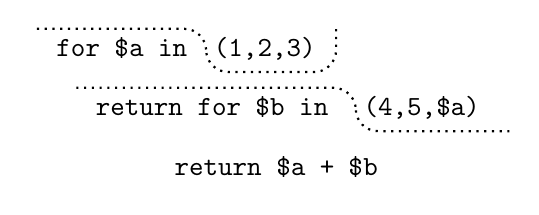
\begin{tikzpicture}
\node at (0,0) [label=right:\texttt{for \$a in}]{};
\node at (2,0) [label=right:\texttt{(1,2,3)}]{};
\node at (0.5,-0.75) [label=right:\texttt{return for \$b in}]{};
\node at (3.9,-0.75) [label=right:\texttt{(4,5,\$a)}]{};
\node at (1.5,-1.5) [label=right:\texttt{return \$a + \$b}]{};
\draw[thick,dotted,rounded corners=8pt]
(0,0.25) -- (2.15,0.25) -- (2.15,-0.3) -- (3.8,-0.3) -- (3.8,0.25) ;
\draw[thick,dotted,rounded corners=8pt]
(0.5,-0.5) -- (4.05,-0.5) -- (4.05,-1.05) -- (6,-1.05);
\end{tikzpicture}
\end{figure*}

As can be seen, the iterator sequence for the inner loop is evaluated in the
scope of the outer loop, and a new scope is not started until this iterator
sequence has been evaluated. Otherwise one could risk overwriting variables in
the iterator sequence when binding variables in the new scope.

Furthermore, a FLWOR construct may consist of several \texttt{for}- and
\texttt{let}-clauses in any order -- and each of these clauses may contain
several variable bindings. For example, the following is a valid XQuery
FLWOR expression:

\begin{center}
\begin{tabular}{l}
\texttt{for \$a in (1,2), \$b in (3,4) let \$c := 5, \$d := 6} \\ \quad
  \texttt{return \$a + \$b + \$c + \$d} \\
\end{tabular}
\end{center}

However note that semantically this expression is equivalent to:

\begin{center}
\begin{tabular}{l}
\texttt{for \$a in (1,2) return} \\ \quad
  \texttt{for \$b in (3,4) return} \\ \quad \quad
    \texttt{let \$c := 5 return} \\ \quad \quad \quad 
      \texttt{let \$d := 6 return} \\ \quad \quad \quad \quad 
        \texttt{\$a + \$b + \$c + \$d} \\
\end{tabular}
\end{center}

The latter seems significantly less complex to parse, since this query embodies
no less than \emph{four} individual FLWOR expressions, each with one and only
one \texttt{for}- or \texttt{let}-clause. This raises the question, could it be
benefitial to rewrite complex FLWOR expressions into a simpler form? This
question is addressed in section \ref{sect:method:ast_rewrite} on page
\pageref{sect:method:ast_rewrite}.

\subsection{Full Text Extensions}
\label{sect:theory:xquery:fulltext_ext}
XQuery is by nature a structural query language -- that is, queries are based on
document/data structure and not on content. The full-text extensions to XQuery
reduces the smallest unit of an XML document to single words instead of nodes.
Additionally, they add sophisticated tools such as stemming, thesaurus, and
scoring variables.

Technically, the \verb!ftcontains! operator applies tokenisation of the first
operand, and searches for a match with the second operand among the tokens. It
allows specifying match options like stemming, thesaurus, etc to a second
operand modifying the criteria for finding a match. A full list of match
options are described in \cite{w3c01}.

For example, consider the following example:
\begin{center}
\begin{tabular}{l}
\texttt{for \$b in /books/book} \\
\texttt{where \$b/title ftcontains ("dog" with stemming case sensitive)} \\ \quad\quad\quad
\texttt{ftand "cat"} \\
\texttt{return \$b/author}
\end{tabular}
\end{center}
This will match any \texttt{book}-node where the \texttt{title}-node contains a word with the stem ``dog''.
Further, the word must be in lower case, and the word ``cat'' must reside inside the same node. The query will
return the \texttt{author}-node of these \texttt{book}-nodes. 

\subsection{XQuery Core}
\label{sect:theory:xquery:XQcore}
XQuery Core is a less powerful but semantically equivalent language for expressing
XQuery queries. XQuery Core as well as the process of normalising regular
XQuery to XQuery Core is described in the document ``XQuery 1.0 and XPath 2.0
Formal Semantics''\cite{xquery_semantics}.

The goal of this subset language is to simplify queries and remove syntactic sugar,
leaving only the essential semantics without loss of expressiveness.
This is useful for optimization routines and translations into new types of
queries, for example relational algebra or SQL.

The process of normalisation is described through a rich set of mapping
rules. These are documented in detail in \cite{xquery_semantics} and will not be reiterated here.
However we will examine some important examples.

First, however, it is important to take note of the syntax of the mapping
rules, as described in \cite{xquery_semantics}, section 3.2.2. 
 
\begin{figure}[!h]
  \centering
$
[Object]_{Subscript}, premises == Mapped Object
$
  \caption{Mapping rules syntax}
  \label{figure:xquery:mapping_rules}
\end{figure}

Consider figure \ref{figure:xquery:mapping_rules}. Here, the left-hand side of the
equality symbol (==) denotes the original object to be rewritten. The
subscript indicates the type or kind of the object to be mapped, and/or
additional information to be passed between mapping rules. The right-hand side
denotes the rewritten object.

\subsubsection{Rewriting FLWOR expressions}
\label{sect:theory:xquery:core:rewriting_flwor}
\begin{figure}[!h]
\centering
[\texttt{for \$}$VarName_1$ $OptTypeDeclaration_1$ $OptPositionalVar_1$ \texttt{in} $Expr_1$\texttt{,}
\ldots, \texttt{\$}$VarName_n$ $OptTypeDeclaration_n$ $OptPositionalVar_n$ \texttt{in} $Expr_n$
$FormalReturnClause]_{Expr}$ \newline
$==$ \newline
\texttt{for \$}$VarName_1$ $OptTypeDeclaration_1$
$OptPositionalVar_1$ \texttt{in} $[Expr_1]_{Expr}$ \texttt{return} \texttt{\ldots for \$}$VarName_n$
$OptTypeDeclaration_n$ $OptPositionalVar_n$ \texttt{in} $[Expr_n]_{Expr}$ \texttt{return}
$[FormalReturnClause]_{Expr}$
  \caption{XQuery FLWOR expression to XQuery Core mapping rule}
  \label{figure:xquery:flwor_mapping_rule}
\end{figure}

The mapping rule for FLWOR \texttt{for}-clause expressions can be seen in figure
\ref{figure:xquery:flwor_mapping_rule}. The mapping rule for \texttt{let}-expressions is
similar and omitted for brevity, however they are also normalised into several nested bindings.

\begin{figure}[!h]
\centering
$[$\texttt{where} $Expr_1 FormalReturnClause]_{Expr}$ \newline
$==$ \newline
\texttt{if(}$[Expr_1]_{Expr}$\texttt{) then }$[FormalReturnClause]_{Expr}$ \texttt{else ()}
  \caption{XQuery \texttt{Where}-clause to XQuery Core mapping rule}
  \label{figure:xquery:where_mapping_rule}
\end{figure}

\begin{figure}[!h]
\centering
$[$\texttt{stable}$?$ \texttt{order by} $OrderSpecList FormalReturnClause]_{Expr}$ \newline
$==$ \newline
$[OrderSpecList]_{OrderSpecList}$\texttt{ return }$[FormalReturnClause]_{Expr}$
  \caption{XQuery \texttt{order by}-clause to XQuery Core mapping rule}
  \label{figure:xquery:orderby_mapping_rule}
\end{figure}

\begin{figure}[!h]
\centering
$[$\texttt{return }$Expr]_{Expr}$ \newline
$==$ \newline
$[Expr]_{Expr}$
  \caption{XQuery \texttt{return} clause to XQuery Core mapping rule}
  \label{figure:xquery:return_mapping_rule}
\end{figure}

Similarly, the mapping rules for \texttt{where}-clauses, \texttt{order by}-clauses and
\texttt{return}-clauses can be seen in figures \ref{figure:xquery:where_mapping_rule},
\ref{figure:xquery:orderby_mapping_rule},
and \ref{figure:xquery:return_mapping_rule}.

For an example of how these rules are applied, consider the following FLWOR
expression:
%\verbatiminput{graph_queries/flwor_rewrite1.xq}
\begin{center}
\begin{tabular}{l}
\texttt{for \$i in (1, 2), \$j in (3, 4)} \\
  \texttt{let \$k := \$i + \$j} \\
  \texttt{where \$k >= 5} \\
   \texttt{return (\$i, \$j)} \\
\end{tabular}
\end{center}

By applying the mapping rules described,  this expression is typically
rewritten to:
%\verbatiminput{graph_queries/flwor_rewrite2.xq}
\begin{center}
\begin{tabular}{l}
\texttt{for \$i in (1, 2) return} \\ \quad
  \texttt{for \$j in (3, 4) return} \\ \quad
    \texttt{let \$k := \$i + \$j return} \\ \quad \quad
      \texttt{if (\$k >= 5) then} \\ \quad \quad \quad
        \texttt{(\$i, \$j)}\\ \quad \quad
      \texttt{else} \\ \quad \quad \quad
        \texttt{()}
\end{tabular}
\end{center}
The corresponding AST graphs can be seen in figures
\ref{tree:ast:flwor_rewrite1} and \ref{tree:ast:flwor_rewrite2}. In particular,
note that multiple \texttt{for}-clauses in a FLWOR expression is rewritten into several
nested FLWOR expressions, and that the \texttt{where}-clause is  rewritten into an
\texttt{if..then..else} expression. 
\newpage
\begin{figure}
\centering
\subfigure[FLWOR AST tree before normalisation]{
 \includegraphics[scale=0.4]{img/graphs/flwor_rewrite1}
\label{tree:ast:flwor_rewrite1}
}
\subfigure[Normalised FLWOR AST tree]{
 \includegraphics[scale=0.4]{img/graphs/flwor_rewrite2}
\label{tree:ast:flwor_rewrite2}
}
\caption{A FLWOR expression before and after normalisation.}
\end{figure}

\subsubsection{Rewriting composite relative path expressions}
A composite relative path expression (for example, \verb!a/b!), can be
rewritten into a \texttt{for}-loop using the mapping rule in
\ref{figure:xquery:relpath_mapping_rule}.

\begin{figure}[!h]
\centering
$[RelativePathExpr / StepExpr]_{Expr}$ \newline
$==$ \newline
\begin{tabular}{l}
\texttt{fs:apply-ordering-mode(} \\ \quad
\texttt{fs:distinct-doc-order-or-atomic-sequence(} \\ \quad\quad
    \texttt{let} \texttt{\$fs:sequence as node()* :=} $[RelativePathExpr]_{Expr}$ \texttt{return} \\\quad\quad
    \texttt{let \$fs:last := fn:count(\$fs:sequence) return} \\\quad\quad
    \texttt{for \$fs:dot at \$fs:position in \$fs:sequence return} \\\quad\quad\quad\quad\quad
       $[StepExpr]_{Expr}$ \texttt{))}
       \end{tabular}
  \caption{Composite relative path expression mapping rule}
  \label{figure:xquery:relpath_mapping_rule}
\end{figure}

Given the trivial example \verb!a/b!, this translates into the following block
of normalised code:
\begin{center}
\begin{minipage}[h]{10cm}
\begin{verbatim}
fs:apply-ordering-mode (
fs:distinct-doc-order-or-atomic-sequence (
  let $fs:sequence as node()* := a return
  let $fs:last := fn:count($fs:sequence) return
  for $fs:dot at $fs:position in $fs:sequence return
    b))
\end{verbatim}
\end{minipage}
\end{center}


Which may seem like a rather verbose representation of such a simple path
expression. In particular, for complex path expressions this may
escalate into rather large rewritten expressions. However, this is a trade-off
to be made for normalisation of such path expressions.


% \subsection{AllMatches}
% \label{sect:theory:xquery:allmatches}
% \begin{itemize}
%   \item http://www.w3.org/TR/xpath-full-text-10/\#AllMatchesSec
%   \item Hva er AllMatches?
%   \item Kobling til fulltekst
%   \item Noen eksempler
%   \item Den store forskjellen med AllMatches er at den minste enheten i et 
%         dokument er et ord og ikke en tekstnode
% \end{itemize}
% om hvis vi bare ignorerer fulltekst uansett. Kunne foreslaatt en tilnarming ala galatex kanskje, som bare
% oversetter greiene til funksjonskall.

\newpage
%Relasjonsalgebra
\section{Relational Algebra}
\label{sect:theory:relAlg}

The relational model for database management was introduced for the first time by Edgar Frank Coddin 1974
(\cite{TDT4225}). It was based on relational algebra which is an offshoot of first-order logic. Several terms are
used when talking about relational algebra (\cite{gordonRussel, newYorkDB, sudarshan}):
\begin{itemize}
\item Set: A mathematical definition for a collection of objects which contains no duplicates
\item Domain: A \textit{set} of atomic values
\item Attribute: A real world role played by a named \textit{domain}
\item Tuple: A collection of \textit{attributes} which describe some real world entity
\item Relation: A \textit{set} of \textit{tuples}
\item Degree: The number of \textit{attributes} a \textit{relation} contains. Sometimes called arity.
\item Cardinality: The number of \textit{tuples} in a \textit{relation}
\item Union compatible: Two relations R and S are union compatible if and only if they have the same
	\textit{degree} and the \textit{domains} of the corresponding \textit{attributes} are the same.
\end{itemize}

\subsection{Primary Operators}
\label{sect:theory:relAlg:primOper}
The primary operators is a set of operators which constitutes the base of an algebra. Other operators can be
defined in terms of the primary ones. If one of the primary operators is excluded, the algebra will loose some of
it's expressiveness. The primitive operators of Codd's algebra are: selection, projection, union, difference,
cross product and rename (later added for the sake of the named relational algebra).

\subsubsection{Selection}
\label{sect:theory:relAlg:selection}
Selection is a unary operator, and is used to obtain a subset of the tuples of a relation that satisfy a select
condition. The resulting relation may have fewer tuples but it will have the same degree as the original relation.
It is sometimes called restriction to avoid confusion with SELECT in SQL. The operator is often symbolized by
\emph{s}igma:
\begin{equation*}
\sigma_{C}(R)
\end{equation*}
Where $R$ is a relation and $C$ is the select condition: a truth value or an expression yielding a truth value.
The expression can be made up of any combination of the logical operators \begin{math}\{ \wedge, \vee,
\neg\}\end{math}. Figure \ref{fig:theory:select} shows an example of a select operation.

\begin{figure}[h]
\centering
\begin{tabular}{lcr}
		\begin{tabular}{|c|c|} \hline
			\multicolumn{2}{|c|}{\textbf{R}} \\ \hline
			\textbf{Letter} & \textbf{Number} \\ \hline
			A & 1 \\ \hline
			A & 3 \\ \hline
			A & 6 \\ \hline
			B & 7 \\ \hline
		\end{tabular}  &
		\begin{math} \sigma _{Letter='A' \wedge Number > 2}(R) = \end{math}
		\begin{tabular}{|c|c|} \hline
			\multicolumn{2}{|c|}{} \\ \hline
			\textbf{Letter} & \textbf{Number} \\ \hline
			A & 3 \\ \hline
			A & 6 \\ \hline
		\end{tabular} 

\end{tabular}
\caption{Example showing the selection operator}
\label{fig:theory:select}
\end{figure}

\subsubsection{Projection}
\label{sect:theory:relAlg:projection}
Projection is also a unary operator, and is used to obtain a subset of the attributes of a relation. The resulting
relation will have an equal or lower degree than the original relation. In the case of duplicates being produced
as a result of omitting some attributes, the resulting relation will have fewer tuples than the original.
\emph{P}i is often used to symbolize the operation:
\begin{equation*}
\pi _{attr}(R)
\end{equation*}
Where $R$ is a relation and $attr$ is the set of attributes to be returned from $R$. Figure
\ref{fig:theory:project} shows an example of a projection. \begin{figure}[h]
\centering
\begin{tabular}{lcr}
	\begin{tabular}{|c|c|c|} \hline
	\multicolumn{3}{|c|}{\textbf{R}} \\ \hline
	\textbf{Let} & \textbf{Num} & \textbf{Sym} \\ \hline
	A & 1 & \% \\ \hline
	B & 1 & \% \\ \hline
	C & 3 & \# \\ \hline
	\end{tabular} &
	\begin{math} \pi _{Num, Sym} (R) = \end{math}
	\begin{tabular}{|c|c|} \hline
	\multicolumn{2}{|c|}{} \\ \hline
	\textbf{Num} & \textbf{Sym} \\ \hline
	1 & \% \\ \hline
	3 & \# \\ \hline
	\end{tabular}
\end{tabular}	
\caption{Exaple showing the projection operator}
\label{fig:theory:project}
\end{figure}

\subsubsection{Union and Difference}
\label{sect:theory:relAlg:unionAndDiff}
Union and difference are two binary operators analogous with union and difference operators in set theory. The
relational algebra version of the operators requires that the relations involved are union compatible.

The union of two relations returns a relation which includes all the tuples that are in either or both of the
original relations. As the result is also a relation, any potential duplicates will be removed. The operation is
commutative, and the returned relation will have the same degree as the two relations involved. A union between
two relations are often symbolized thus:
\begin{equation*}
R \cup S
\end{equation*}
Where $R$ and $S$ are relations.

The difference of two relations R and S is a relation that contains all the tuples that are in R but not in S. The
returned relation will, as was the case with union, have the same degree as the two relations involved. A
difference between relations $R$ and $S$ is written like this:
\begin{equation*}
R - S 
\end{equation*}

\subsubsection{Cross Product}
\label{sect:theory:relAlg:crossProduct}
The cross product operator is sometimes referred to as the cartesian product operator. As with union and
difference, it also stems from set theory. The operator is used to combine all tuples in one relation with all the
tuples from another. The returned relation will have a degree equal the sum of the degrees of each of the original
relations, and a cardinality equal the product of the cardinalities. The operator is commutative and written as a
cross:
\begin{equation*}
R \times S = S \times R
\end{equation*}
Where $R$ and $S$ are relations. Figure \ref{fig:theory:crossproduct} shows an
example of a cross product. \begin{figure}[h]
\begin{tabular}{ccccc}
	\begin{tabular}{|c|} \hline
	\textbf{R} \\ \hline
	\textbf{Let} \\ \hline
	A \\ \hline
	B \\ \hline
	\end{tabular}
	&
	\begin{math} \times \end{math}
	&
	\begin{tabular}{|c|c|} \hline
	\multicolumn{2}{|c|}{\textbf{S}} \\ \hline
	\textbf{Num} & \textbf{Let} \\ \hline
	1 & C \\ \hline
	2 & A \\ \hline
	\end{tabular}
	&
	\begin{math} = \end{math}
	&
	\begin{tabular}{|c|c|c|} \hline
	\multicolumn{3}{|c|}{} \\ \hline
	\textbf{R.Let} & \textbf{S.Num} & \textbf{S.Let} \\ \hline
	A & 1 & C \\ \hline
	A & 2 & C \\ \hline
	B & 1 & C \\ \hline
	B & 2 & A \\ \hline
	\end{tabular}
\end{tabular}
\centering
\caption{An example of cross product.}
\label{fig:theory:crossproduct}
\end{figure}

\subsubsection{Rename}
\label{sect:theory:relAlg:rename}
Rename is a unary operator used to rename a relation and/or a subset of its attributes. The resulting relation
will be equal to the original one in all aspects except maybe some of its name properties. The Greek letter
\emph{r}ho is often used to mark the presence of the rename operator:
\begin{equation*}
\rho _{S}(R)
\end{equation*}
Where $R$ is the relation being renamed, and $S$ is a relational scheme. $S$ is on the form $T _{(a _{1},...a
_{n})}$ for a n-degree relation, where $T$ is the new relation name and $a _{1},...a _{n}$ is the new names for
relation $R$'s attributes from $1$ to $n$. The degree of the scheme must be the same as the degree of the relation
being operated on.

\subsection{Derived Operators}
\label{sect:theory:relAlg:derivedOper}
None of the six primary operators can be expressed as a combination of any of the others. In contrast, some useful
operators can be derived using one or more of the primary ones. Most notably among these are intersection and join.

\subsubsection{Intersection}
\label{sect:theory:relAlg:intersection}
Intersection is the fourth mentioned operator that stems from set theory. It is a binary operator, and the
resulting relation will contain the set of tuples that are in both of the relations operated on. It can be
expressed with the help of the difference operator, and hence require that the input relations are union compatible:
\begin{equation*}
R \cup S = R-(R-S)
\end{equation*}

\subsubsection{Joins}
\label{sect:theory:relAlg:joins}
Joins are a group of operators that all are derived from the primary operators with the cross product as a base.
Among the operators in this group is natural join, theta-join, equi-join, anti-join, semi-join, outer joins and
division. Some of these will be presented in this section.

\paragraph{Natural Join.}
\label{sect:theory:relAlg:naturalJoin}
Natural join is a binary operator that returns a relation consisting of all combinations of tuples in input
relations that are equal on their common attribute names. The result relation will have a degree equal to the sum
of the degrees of the two original relations subtracted the number of common attributes. It is possible to express
natural join as a combination of cross product, projection and selection:

\begin{equation*}
R \bowtie S = \pi_{a_{1},..., a_{n},R.b_{1},...,R.b_{n},c_{1},...,c_{n}}( \sigma _{R.b_{1}=S.b_{1} \wedge ... \wedge R.b_{n}=S.b_{n}}(R \times S))
\end{equation*}

Where $R$ and $S$ are relations, $b_{1},..,b_{n}$ are the common attributes, $a_{1},..,a_{m}$ are the attributes
unique to $R$ and $c_{1},...,c_{k}$ are the attributes unique to $S$. A rename operator can lastly be used to
remove the prefix of the common attributes.

\paragraph{Equi-join and Theta-join.}
\label{sect:theory:relAlg:equiAndThetaJoin}
Theta-join returns a relation which is a combination of all the tuples in the two input relations that satisfy a
condition $C$. $C$ is in the form $a \theta b$, where $a$ is a attribute name from one relation, $b$ is an
attribute from the other and $ \theta $ is a binary operator in the set $ \{ <, \leq , =, \geq , >  \} $. An
equi-join is a theta-join where the binary operator in the condition is the equality operator. Theta-join can be
expressed as a combination of select and cross product:

\begin{equation*}
R \bowtie _{a \theta b}S = \sigma _{a \theta b}(R \times S)
\end{equation*}

\paragraph{Division.}
\label{sect:theory:relAlg:division}
Division in relational algebra can be described as the inverse operator of cross product, in the same way division
and multiplication are inverse in natural numbers calculus -- i.e. they are not inverse if the division gives a
residue:

\begin{equation*}
(R \times S) \div R = S ~~and~~ (R \times S) \div S = R
\end{equation*}

The resulting relation after a division contains the attribute values of the divisor relation that are associated
with every member of the dividend relation (\cite{makeDiv}). The operation may be better explained as a
combination of cross product, projection and difference:

\begin{equation*}
R \div S = \pi _{a_{1},...,a_{n}}(R) - \pi _{a_{1},...,a_{n}}((\pi _{a_{1},...,a_{n}}(R) \times S) - R)
\end{equation*}

Where $R$ and $S$ are relations and $a_{1},...,a_{n}$ are the attributes unique to $R$.

\paragraph{Semi-join.}
\label{sect:theory:relAlg:semiJoin}
Semi-join is a binary operation which returns a relation with the attributes of the first relation, and all the
tuples in this same relation for which there is a tuple in the second relation that is equal on their common
attributes. Semi-join can be described with the projection and natural-join operators:

\begin{equation*}
R \ltimes S = \pi _{a_{1},...,a_{n}}(R \bowtie S)
\end{equation*}

Where $R$ and $S$ are relations, and $a_{1},...,a_{n}$ are the attributes unique to $R$.

\paragraph{Anti-join.}
\label{sect:theory:relAlg:antiJoin}
The anti-join operator is very similar to the semi-join operator (and is also sometimes referred to as the
anti-semi-join), except that it returns all the tuples in the first relation for which there is not a tuple in the
other relation on their common attributes. It can be described with help of semi-join and difference:

\begin{equation*}
R \rhd S = R - R \ltimes S
\end{equation*}

Where $R$ and $S$ are relations.

\paragraph{Outer Joins.}
\label{sect:theory:relAlg:outerJoin}
The outer joins works in many ways as the natural join, except the resulting relation will include some extra
tuples based on one or both of the input relations. The right outer join $(\times=)$ will return a relation with
all the tuples from a natural join between the first (left) and the second (right) relation, but also the tuples
from the right relation that did not match any tuples from the left one on their common attributes. These extra
tuples will have the value NULL in the result relation for all attributes that were unique to the left one. The
left outer join $(=\times)$ is analogous with the right version, the only difference is that the extra tuples will
be based on the left input relation. The result relation of a full outer join $(=\times=)$ will have extra tuples
based the ones that did not find a match in both input relations.

\newpage
% State of the art, nåværende teknologi og implementasjoner
\section{Current state of XQuery}
\subsection{General}
\subsection{Implementations with full-text extensions}
\subsubsection{Quark / TexQuery}
\newpage
\section{ANTLR}
ANTLR, Another Tool for Language Recognition, is a parser generator under a three clause BSD-license (\cite{antlrorg}).  It is a successor of PCCTS, sometimes called ANTLR v1, and the latest version is ANTLR v3. PCCTS was developed by Professor Terrence Parr of the University of San Francisco, now the primus motor behind ANTLR.

ANTLR generates recursive-decent recognizers that utilizes predicated LL(*) -- an extension to LL(k) that uses arbitrary lookahead to make decisions. LL parsers are often said to be more intuitive and easier for humans to read than e.g. LALR parsers. This is supported by the fact that most hand written parsers are LL parsers. ANTLR supports multiple target languages, including Java. There are generally three types of recognizers ANTLR can generate: lexers, parsers and tree parsers/walkers.

\subsection{LL(*)}
The LL(*) parsing strategy is a strategy unique to ANTLR, invented by Terrence Parr for ANTLR v3. It is much more powerful than traditional LL(k) parsing (\cite{definitiveAntlr}), because it is not limited to a finite amount of lookahead. It enhances the LL decision's predictive capabilities, but does not by means alter the recursive decent parsing strategy.  By automatically doing left-factoring LL(*) allows developers to write more natural and human readable grammar. If a grammar is specified as LL(k), LL(*) will degenerate into LL(k) for this grammar. A decision is LL(*) if a DFA exist that recognizes the decision's exact lookahead language and has the following (\cite{definitiveAntlr}):
\begin{itemize}
\item No unreachable states
\item No dangling states, i.e. states that cannot reach an accept state
\item At least one accept state for each alternative.
\end{itemize}
All alternatives have a lookahead language, and if the lookahead languages of the alternatives are disjoint, the decision is LL(*). Except for not having a finite lookahead, LL(*) differs from LL(k) with backtracking in that it is looking ahead with the DFA, and not the whole parser. A thorough description of LL(*) can be found in \cite{lookahead}.

\subsection{Grammar Specification}
\label{sect:antlr:grammarSpec}
The grammar is specified in a type of extended Backus-Naur form (EBNF), where the extension from BNF consists of the Kleene operators $?$, $ +$ and $\ast$, and the not-operator $\sim$.  In addition, ANTLR introduces some types of predicates, namely validating, hoisting and gated semantic predicates and syntactic predicates. Validating and disambiguating semantic predicates is on the form \verb!{sem. predicate}?!, gated semantic predicates is on the form \verb!{sem. predicate}?=>! and syntactic predicates is on the form \verb!(syn. pred.)=>!.

Member methods and variables of the parser can be placed in a \verb!@members{! members \verb!}! construct, and the corresponding \verb!@lexer::members{! members \verb!}! for the lexer. Actions specified in the target language can be inserted at appropriate places in the production rules wrapped in \verb!{! and \verb!}!. 

Lexer productions and token names start with a capital letter, and parser productions do not. It is possible, and even common, to specify both the lexer and parser grammar in one file, thus ANTLR will determine which productions that belong to the lexer and the parser respectively by looking at the case of the first letter in the name of the production rules. An example of ANTLR grammar can be seen in figure \ref{code:simpleGrammar}. This grammar will generate a parser that recognizes input such as "John is 37 years old".
\begin{figure}[h!]
\begin{verbatim}
NAME     : ( 'a'..'z' | 'A'..'Z')+;  
AGE      : ('1'..'9')? ('1'..'9'|'0');
sentence :  NAME ' is ' AGE  ' years old';
\end{verbatim}
\caption{ANTLR grammar example}
\label{code:simpleGrammar}
\end{figure}

\subsection{Lexer}
Lexers generated by ANTLR is by default a class derived from \verb!Lexer! (in the \verb!org.antlr.runtime! package) with additional per lexer rule methods for matching incomming character data. The lexer depends upon a input module that implements the \verb!CharStream! (e.g. \verb!AntlrStringStream!) interface which defines the method \verb!public int LT(int k)!. This method returns the character in the input stream \verb!k! positions from the current position. The method \verb!public Token nextToken()! in the lexer will generate and return the next token found by the lexer in the character stream. An overview of this method can be seen in figure \ref{fig:nextToken}, where \verb!Lexer! is \verb!org.antlr.runtime.Lexer! and \verb!TestLexer! is the lexer generated by a fictional grammar \verb!Test!.

\begin{figure}[h]
\centering
\begin{tabular}{|l|l|l|} \hline
\textbf{Lexer} 				& \textbf{TestLexer} 			\\ \hline
\verb!CharStream input;!		& 					\\
					&					\\
\verb!nextToken(){!			&					\\
\verb!   token = NULL;!			&					\\
\verb!   pos = input.position!		&					\\
\verb!   text = NULL;!			&					\\
					& \verb!mTokens{!			\\ 
					& \verb!   _type = "predict type"!	\\
					& \verb!   input.updatePosition()!	\\
					& \verb!   this.type = _type;!		\\
					& \verb!}!				\\
\verb!   if(token == NULL){!		&					\\
\verb!     emit(){!			&					\\
\verb!        t=new Token(type, pos,! 	&					\\
\verb!            input.position, input);!&					\\ 
\verb!        t.setText(text)!		&					\\
\verb!        emit(t){!			&					\\
\verb!          token=t;}!		&					\\
\verb!     }!				&					\\
\verb!   }!				&					\\
\verb!   return token;!			&					\\
\verb!}!				&					\\ \hline
\end{tabular}
\caption{Pseudocode showing how the lexer generates tokens.}
\label{fig:nextToken}
\end{figure}
Unless explicitly defined the tokens will hold the text they have matched as \verb!input!, \verb!startPosition! and \verb!endPosition!. It is also worth noticing that \verb!token! is set to \verb!NULL! for each token request, and a token will only be generated by \verb!nextToken()! if \verb!token! still has the value \verb!NULL! after the generated part of the lexer has decided which token to match.

When the lexer is to predict which type of token it should return (\verb!"predict type"! in figure \ref{fig:nextToken}), it peeks into the input character stream as many positions ahead needed to disambiguate the alternatives and make a decision. However, for e.g. to easily be able to define keywords, some ambiguous alternatives are allowed. ANTLR will then choose between the alternatives following some simple rules:
\begin{itemize}
\item An explicit expressed character sequence is chosen before an implicit one.
\item A longer sequence is chosen before a shorter one.
\item A production declared before another is chosen first.
\end{itemize}
These rules are ranked, and ANTLR will only use as many of them needed to differanciate the alternatives. Syntactic and semantic predicates will also make an impact on the decisionmaking as seen later. Figure \ref{fig:grammarPrec} shows a grammar with ambiguous alternatives, a simplified version of the code generated can be seen in figure \ref{fig:codeGenerated} where you can see that the parser will choose \verb!AB! before \verb!A! (and thus \verb!A B!) and \verb!A! before \verb!ANY!.
\begin{figure}[h!]
\begin{verbatim}
A       : 'a';
B       : 'b';
AB      : 'ab';
ANY     : ('a'..'z')+;
\end{verbatim}
\caption{Grammar showing the precidence among rules}
\label{fig:grammarPrec}
\end{figure}

\begin{figure}[h!]
\begin{verbatim}
int alt = 4;
if(LA(1) == 'a')
      if(LA(2) == 'b')
            if(LA(3) >= 'a' && LA(3) <= 'z')
                  alt = 4;
            else
                  alt = 3;
      else
            alt = 1;
else if(LA(1) == 'b')
      if(LA(2) >= 'a' && LA(2) <= 'z')
            alt = 4;
      else
            alt = 2;
else if(LA(1) >= 'c' && LA(1) <= 'z')
      alt = 4;
else
      throw new NoViableAltException();
\end{verbatim}
\caption{Example of how ANTLR predicts token type.}
\label{fig:codeGenerated}
\end{figure}
Production rules declared with the keyword \verb!fragment! are rules that never will be implicitly considered as an alternative. Fragment rules depend upon being referenced by other rules, fragment or not.
If the lexer grammar is so big that it may not compile, ANTLR will substitute the inline DFAs with DFA objects for prediction. These objects are implemented as a set of transition tables. More about the DFA objects can be found in \cite{antlrCodeGen}.

\subsection{Parser}
\label{sect:antlr:parser}
The parser generated by ANTLR is very much analogous with the lexer. By default the parser will be derived from \verb!org.antlr.runtime.Parser!. In addition to the methods and variables inherited, the generated parser will contain one method per production rule in the parser grammar. The parser does not have one defined "starting rule", thus, each method will have a prediction algorithm similar to \verb!mTokens()! in the lexer. As with the lexer, the algorithm peeks into the input stream as many tokens forward needed to differentiate between the alternatives. The parser takes a object that implements \verb!TokenStream! as input, which again takes a \verb!TokenSource! (the base class of \verb!Lexer!) as input. \verb!TokenStream! contains a method \verb!LT(int k)!, and classes that implements this interface often include a method \verb!LA(int k)! which returns the type of the token returned by the other method. \verb!CommonTokenStream! is a simple implementation of \verb!TokenStream!, and recomended by the ANTLR Community (\cite{antlrorg}) in most cases. The first time the \verb!LA(int k)! method of \verb!CommonTokenStream! is called a buffer of tokens will be filled by calling the lexer's \verb!nextToken()! until it returns \verb!Token.EOF! -- the end of the input. This means that before the parser starts to try matching production rules, the lexer will be finished creating tokens. Parsing will commence by calling the method created for the top-most production in the grammar, which in the case of XQuery with full text extension is \verb!module()!.

\subsection{Generating an Abstract Syntax Tree}
\underline{\textbf{\LARGE //TODO}}
\\
\begin{itemize}
\item Hvordan generer antlr AST 
\item hvordan spesifisere annet en default 
\item rotnode (\^{})
\item imaginary tokens
\item unnlate tokens (!)
\item rewrite rules (->)
\end{itemize}
By default, ANTLR will not generate an AST from the grammar specification.
However, by setting the \verb!output! option value to \verb!AST! in the grammar
header, ANTLR will generate a simple ``flat'' linked list consisting of all the
parsed tokens in the input. 

This flat AST can be structured by adding operators and rewrite rules to tell
ANTLR which tokens to use as root nodes in productions, and which to leave out
of the AST entirely. There are two primary operators for AST structuring, hat
(\^{}) and exclamation mark (!). These operators are postfixed to tokens to
promote them to root nodes and exclude them completely from the AST,
respectively. Figure \ref{code:astOperators} shows an example where the
paranthesis would be excluded from the AST, and the \verb!PLUS! token
would be promoted to root node with two \verb!expr! children.

\begin{figure}[h!]
\begin{verbatim}
sum : '('! expr PLUS^ expr ')'!;
\end{verbatim}
\caption{Simple AST structuring operators example}
\label{code:astOperators}
\end{figure}

Additionally, ANTLR provides the commodity of rewrite rules for tailoring AST
generation. Figure \ref{code:astRewriteRules} shows an example with a rule for
an if-statement. The ``arrow'' (->) marks the start of the rewrite rule. The hat
(\^{}) operator indicates that the first token in the list should be promoted to
root node. There is no need to use exclamation marks as simple omission will
leave unwanted tokens out of the AST. Also note that variables can be used
exactly like in grammar predicates.

\begin{figure}[h!]
\begin{verbatim}
if : 'if' expr 'then' s1=stmt 'else' s2=stmt 'endif'
     -> ^(IFEXPR expr $s1 $s2);
\end{verbatim}
\caption{Usage of simple AST rewrite rules}
\label{code:astRewriteRules}
\end{figure}

Sometimes it may be necessary to customize the AST by adding custom fields to
the nodes or performing certain operations on them not supported by the built-in
tree representations. This can be done by subclassing the BaseTree (or
CommonTree) classes as well as adding a custom tree adaptor class, and setting
the option \verb!ASTLabelType=MyCustomTreeClass! in the grammar file header.

\subsection{Semantic Predicates}
\label{sect:antlr:semantic_preds}
Even though LL(*) allows the parser to scan arbitrarily far forward for any symbol or sequence of symbols to distinguish alternatives, it still has some weaknesses - particularly so when it comes to recursive rules. Semantic predicates are boolean expressions evaluated during runtime used to specify the semantic validity of an alternative. Predicate in this case simply means conditional, and the term semantic implies you are talking about arbitrary boolean expressions rather than a syntactic condition.  As previously mentioned, ANTLR provides three types of semantic predicates:
\begin{itemize}
\item Disambiguating semantic predicates; which disambiguate syntactically identical alternatives.
\item Gated semantic predicates; which can dynamically turn on and off parts of the grammar.
\item Validating semantic predicates; which throw a recognition exception if the predicate fails.
\end{itemize}

\subsubsection{Validating Semantic Predicates}
If the expression being evaluated in a validating semantic predicate yields $false$, an exception is thrown, expressing that a semantic predicate has failed. These predicates are never included in the decision-making process. Validating semantic predicates can be very handy in cases where e.g. you want to restrain the possible values a tokens can have, or to check if a variable is being referenced before its declaration. An example of a validating semantic predicate can be seen in figure \ref{code:validateSemantic}.

\begin{figure}[h!]
\begin{verbatim}
expr    : N {Integer.parseInt($N.getText()).intValue() < 7}?
        | . . .
        ;
\end{verbatim}
\caption[Validating semantic predicate.]{A Validating semantic predicate checking if the number value of \texttt{N} is less than $7$.}
\label{code:validateSemantic}
\end{figure}
As can be seen from this example, a semantic predicate is simply any kind of boolean Java expression. This is a flexible solution, because the boolean expression can be wrapped in a method with boolean return type, which for example then can be placed inside a @members { } clause in the grammar file, or even as a static method in an external class. This makes it possible to add complex grammar logic without
disturbing grammar brevity, if necessary.

\subsubsection{Disambiguating Semantic Predicates}
Disambiguating semantic predicates are hoisted into the prediction decisions of the LL(*) recognizer, but only if no decision can be made by syntax alone. There are generally two cases where these types of predicates are really useful: when a property of a token must dictate how the parser interprets it, and when a surrounding construct or some runtime information should alter how the parser matches the current construct. In most cases when a validating semantic predicate is applied, it can be transformed into a disambiguating semantic predicate. This will result in a syntax error instead of an exception if the predicate evaluates to $false$.

To fully resolve a non-determinism with disambiguating semantic predicates, all alternatives that contribute to the non-determinism will have to be covered, as seen in figure \ref{code:disambigSemantic}. The DFA generated in figure \ref{code:disambigSemantic} is illustrated in figure \ref{fig:dfaDisambiguate}.

\begin{figure}[h!]
\begin{verbatim}
expr      : {pred1}? A 
          | {pred2}? A
          ;
\end{verbatim}
\caption{Disambiguating semantic predicates.}
\label{code:disambigSemantic}
\end{figure}

\begin{figure}[!h]
  \centering
    \includegraphics[scale=0.6]{img/disambigsemantic}
  \caption{The DFA of figure \ref{code:disambigSemantic}}
  \label{fig:dfaDisambiguate}
\end{figure}
As mentioned earlier, ANTLR hoists disambiguating semantic predicates into the state where the alternative prediction is made, which can be illustrated by the fact that the grammar inn figure \ref{code:disambigSemanticHoist} also yields the DFA shown in figure \ref{fig:dfaDisambiguate}. This includes only the predicates visible at the left edge of the production rule. 
\begin{figure}[h!]
\begin{verbatim}
expr      : a 
          | b
          ;
a         : {pred1}? A ;
b         : {pred2}? A;
\end{verbatim}
\caption{Hoisted disambiguating semantic predicates.}
\label{code:disambigSemanticHoist}
\end{figure}
Predicates implicitly specify precedence among the alternatives, where an earlier specified alternative has precedence over a later one. If both \verb!pred1! and \verb!pred2! would evaluate to true in figure \ref{code:disambigSemantic}., the first \verb!A! would be matched. In the case of only the first $n-1$ non-deterministic alternatives among $n$ are covered by a semantic predicate, the $n$th alternative would be covered with a \verb!{true}?! predicate. However, if this uncovered alternative was places first, it would be covered by a predicate that is the complement of the union of the following $n-1$ predicates.

\subsubsection{Gated Semantic Predicates}
Gated semantic predicates are used when it is desirable to turn parts of a grammar on or off based on runtime information. The predicate will be hoisted into the decision even if the decision is deterministic by considering syntax alone. The difference between gated and disambiguating semantic predicates is that decisions use disambiguating semantic predicates only when syntax alone is insufficient to distinguish between alternatives. Figure \ref{code:gatedSemantic} shows an example of a gated semantic predicate, the resulting DFA is illustrated in figure \ref{fig:dfaGated}, showing how the predicate is hoisted even with no syntactic ambiguity.

\begin{figure}[h!]
\begin{verbatim}
expr      : a 
          | b
          ; 
a         : A;
b         : {pred}?=>B;
\end{verbatim}
\caption{Gated semantic predicate.}
\label{code:gatedSemantic}
\end{figure}

\begin{figure}[!h]
  \centering
    \includegraphics[scale=0.6]{img/gatedsemantic}
  \caption{The DFA of figure \ref{code:gatedSemantic}}
  \label{fig:dfaGated}
\end{figure}

\subsection{Syntactic Predicates}
Syntactic predicates are similar to semantic predicates except that they specify the syntactic validity of applying an alternative rather than the semantic validity. As with the semantic predicates their syntactic counterparts alter the parse based upon information available at runtime, but the only information the syntactic predicates use are future input symbols.  Both syntactic predicates and LL(*) support arbitrary lookahead, but whereas LL(*) uses a DFA to examine the future input symbols, the predicates use a pushdown machine, making them capable of recognizing more complicated structures in the lookahead than DFAs. Syntactic predicates are especially useful to specify the precedence between to ambiguous alternatives, or when LL(*) cannot handle the grammar the way you would like to write it.

When used to disambiguate between alternatives, ANTLR will try the alternatives in order. The alternative whose predicate is the first to return true, is the one chosen ("if it looks like A, it is A"). In its simplest form, syntactic predicates can be used to look ahead an arbitrarily number of symbols, to check if they match the symbols specified in the predicate. In a case like this ANTLR rewrites the predicate to a gated semantic predicate, an example of this is the grammar in figure \ref{code:syntactic} being translated to the equivalent grammar of figure \ref{code:translatedSyntactic}.

\begin{figure}[h!]
\begin{verbatim}
expr      : (A)=> A 
          | B
          ; 
\end{verbatim}
\caption{Syntactic predicate.}
\label{code:syntactic}
\end{figure}
\begin{figure}[h!]
\begin{verbatim}
expr      : {input.LA(1)==A}?=>A 
          | B
          ; 
\end{verbatim}
\caption{Translated syntactic predicate}
\label{code:translatedSyntactic}
\end{figure}

In more complex cases, syntactic predicates are implemented as disambiguating semantic predicates that invoke parser backtracking methods. These methods compare the input stream with the symbols specified in the predicate. If the stream and the symbols match, the method returns true, and the input stream is rolled back to the place where the comparing started. Such a case is exemplified by figure \ref{code:complexSyntactic}, where with an input such as "((a))" ANTLR will try the second alternative, succeed, backtrack, before telling the parser to choose this alternative.
\begin{figure}[h!]
\begin{verbatim}
expr      : (simple)=> simple ';'
          | (recur)=> recur ';'  
          | simple '!'
          ;
simple    : '(' ID ')';
recur     : '(' recur ')'
          | ID
          ;
ID        : ('a'..'z')+;
\end{verbatim}
\caption{A syntactic predicate which may backtrack}
\label{code:complexSyntactic}
\end{figure}

%\newpage
%\mbox{}

%Relasjonsalgebra
\chapter{Architectual Decisions}
\label{chapter:method}
Because we decided to create the parser with a generator, different alternatives of such tools had to be evaluated. In this chapter we will document this process. Further, we will present other decisions we made before implementating the recognizer. This constitutes the choice of licence and means testing the system. Finally we will present the problem with the ambiguous terminals and evaluate different lexer strategies that would solve this.

\section{Parser construction}
Writing a parser from scratch was ruled out early for being too time consuming.
Instead it was decided to use tools for compiler and parser construction to
generate a parser from the XQuery 1.0 and XPath 2.0 grammar  
specifications\cite{w3c01} developed by the W3C.

Some important requirements were taken into account when evaluating these
alternatives. Specifically, the generator must:
\begin{itemize}
  \item generate Java source code for the parser
  \item be able to generate an LL(1) (or LL(k)) parser, because the grammar  
  specification is given by W3C in LL(k)
  \item be licensed liberally, either GPL or BSD, or an equivalent license
  approved by OSI
\end{itemize}

\subsection{Evaluated alternatives}
\label{sect:method:alternatives}
\subsubsection{JFlex/CUP}
JFlex and CUP is a versatile combination consisting of JFlex which is a lexer
generator, and CUP which is a parser generator. These tools can be interfaced to
generate a complete parser with a separate lexical analyzer.

JFlex and CUP produces only LALR parsers, and since the W3C has specified an
LL(1) grammar for XQuery 1.0 and XPath 2.0, the combination of JFlex and CUP was
rejected from this project. Additionally, some basic occurence operators such as
*,+ and ? is not supported by CUP.

In the light of this decision, it is important to note that a large amount of
work can be avoided by rejecting a LALR parser generator solution for this
project. Consider the examples in figure \ref{code:parsers:lalr} and
\ref{code:parsers:ll} and compare it to the reference grammar specification in
figure \ref{code:parsers:w3c}.

\begin{figure}[h!]
\begin{verbatim}
LetClause : "let $" LetBindings_
LetBindings_ : VarName OptTypeDeclaration_ ":=" ExprSingle
        | VarName OptTypeDeclaration_ ":=" ExprSingle
        "," "$" LetBindings_
\end{verbatim}
\caption[LALR grammar example]{LALR grammar example from the Pathfinder project
(see section \ref{sect:soa:pathfinder})}
\label{code:parsers:lalr}
\end{figure}

\begin{figure}[h!]
\begin{verbatim}
letClause : LET varBinding (COMMA varBinding)*

varBinding : (DOLLAR varName typeDeclaration? | 
             SCORE DOLLAR varName )
             ASSIGN exprSingle
\end{verbatim}
\caption[LL grammar example]{LL grammar example, actual code used in this project}
\label{code:parsers:ll}
\end{figure}

\begin{figure}[h!]
\begin{verbatim}
LetClause ::=  (("let" "$" VarName TypeDeclaration?) 
 				| ("let" "score" "$"  VarName)) ":=" ExprSingle ("," 
 				(("$" VarName TypeDeclaration?) 
 				| FTScoreVar) ":=" ExprSingle)*
\end{verbatim}
\caption{ W3C reference grammar example }
\label{code:parsers:w3c}
\end{figure}

Obviously, the LALR-grammar has suffered an extensive rewrite into a recursive
rule to compensate for the lack of support for occurence indicators. The LL
example stands out as clear and readable, even more so than the W3C
grammar specification.

In the case of JFlex/CUP, building abstract syntax trees is a process that must
be done manually by adding action code snippets to the grammar. This is
unfortunate for several reasons - it dilutes the grammar and decreases
readability and clarity.


\subsubsection{JavaCC}
JavaCC could have been a viable alternative as it produces LL(k) parsers,
however compared to Antlr its grammar specification syntax deviated more
from the W3C EBNF syntax, meaning that the grammar would have had to be
extensively rewritten. However, JavaCC supports the same occurence indicators
used in the XQuery grammar specification. Figure \ref{code:parsers:javacc} shows
a grammar fragment translated to JavaCC syntax, compare to the original grammar
in figure \ref{code:parsers:w3c}.

\begin{figure}[h!]
\begin{verbatim}
void letClause() :
{ }
{
    <LET> varBinding() (COMMA varBinding())*
} 

void varBinding()
{ }
{
    (<DOLLAR> varName() typeDeclaration()? | 
     <SCORE> <DOLLAR> varName() )
     <ASSIGN> exprSingle()
}
\end{verbatim}
\caption{ JavaCC reference grammar example }
\label{code:parsers:javacc}
\end{figure}

For AST construction, JavaCC requires the use of preprocessor tool known as  
JJTree. This tool will parse the grammar and insert tree building actions where
appropriate. 

\subsubsection{ANTLR}
ANTLR is a renowned tool for parser generation, and can generate LL(*) parsers.
Additionally, ANTLR accepts a grammar specification syntactically very close to
the EBNF used by the W3C. This is the parser generater chosen for our project,
based on the criteria outlined in this section.

The details of this parser generator is outlined in chapter \ref{sect:antlr}.

\section{Debugging}
\label{sect:method:debugging}
There are several approaches to debugging. ANTLRWorks \cite{antlrwrks00} is a
simple tool for writing, testing and debugging Antlr grammars. The debugging
interface is useful in that it draws a realtime step-by-step parse tree as the
input is being parsed, as well as displaying a list of parser events.
ANTLRWorks also helps eliminate grammar nondeterminisms by drawing the syntax
diagram associated with a grammar and highlighting nondeterministic paths. A
big drawback, though, is as the grammar grows bigger, the application tends to
become unstable.    

When working properly, ANTLRWorks is a great tool for debuging the parser, but
no so much for the lexer. It will show the tokens returned to the parser, but
no information or decision path indicating the reason for returning just that
token. A more appropriate tool for such a task would be the standard debuging
environment in Eclipse (\cite{eclipse}).    

% Method / Testing
\section{Testing}
\label{sect:method:testing}
To improve quality insurance in this projects, it was decided to systematically
write tests for new features as well as perform coverage testing for comparison
with existing implementations. This section will outline the various test
methods used in this project. Also see section \ref{sect:results:tests}, where
the test results are presented.

\subsection{gUnit}
\label{sect:method:gUnit}
Unit testing can be a powerful tool for asserting functionality and can be a
helpful aid in debugging and prevention of regression errors.  For unit testing the
grammar specification, gUnit \cite{gunit00} was employed. This tool uses a
syntax similar to Antlr itself, however instead of defining productions, one
defines a set of inputs for some rule, as well as the expected result. Consider
this example:

\begin{Verbatim}
gunit XQFT;
@header{package no.ntnu.xqft.parse;}

piTarget: // Test piTarget rule

    // Any case permutation of 'XML' must fail
    "Xml" FAIL
    "XMl" FAIL
    "XML" FAIL
    "XmL" FAIL
\end{Verbatim}

This is a complete input file for gUnit, and will automatically discover the
classes XQFTLexer and XQFTParser in the package no.ntnu.xqft.parse. gUnit will
then proceed to invoke the lexer with ``Xml'', ``XMl'', ``XML'', and ``XmL'' as
input, and pass the lexer to an instance of XQFTParser and execute the production
piTarget. For all these inputs, it will assert that the parser emits an error
(i.e it must fail to pass the test).

In case of a test where the parser should not fail, the syntax is as follows:
\begin{Verbatim}
forClause:
	"for $a in document(\"abc.xml\")/a/b/text()" OK
\end{Verbatim}
Here gUnit will assert that the parser will not fail for the given inpu (i.e it
must not fail to pass the test).

gUnit is also capable of parsing abstract syntax trees built by the generated
parser, but this feature has not been used in this project.

\subsection{jUnit}
In addition to the gUnit tests for the grammar, jUnit was used to write unit tests for
the additional classes needed for this parser. In particular, the classes
related to scoping and symbol tables. Here is one example, asserting that the
setParent() method in the scope class works as expected:
\begin{Verbatim}
    @Test
    public void testSetParent() {
        this.scope = new Scope();
        Scope tmp = new Scope();
        this.scope.setParent(tmp);
        assertEquals(this.scope.getParent(), tmp);
    }
\end{Verbatim}

\subsection{Manual Coverage Tests}
Finally, we employed manual tests for running the complete XQuery Test Suite\cite{w3c05}
as a benchmark for XQuery compliance. Specifically, we simplified this approach
into counting any test query accepted by the parser as passed. Since the parser
does not generate any results from queries, it was impossible to run a
comparison to the given expected results.

The test suite consists of a total of 12584 different queries with a
corresponding set of expected output. These tests span a large amount of XQuery
functionality. Out of these tests, a total of 10363 tests are applicable for
this project. These tests are categorized as scenarios: \emph{standard}, 
\emph{parse-error}, and \emph{trivial}. The remaining tests are only possible to
perform in run time, and are thus not applicable for this parser at this time.
\section{Licensing}
\label{sect:method:licensing}
One requirement for the parser is to license the produced software under a
permissive open source license. Several such liberal licenses exist, however here we
shall review a short selection of popular and widely adopted licenses, and
choose one for this project. These licenses have been gathered from the Open
Source Initiative (OSI) website\cite{osi_website}, from the category
``\emph{Licenses that are popular and widely used or with strong communities}''.

\subsection*{GPLv2 -- General Public License version 2}
The GPL license is a widely adopted license known for its reciprocality and
enforcement of ``copyleft''\footnote{http://www.gnu.org/copyleft/} to ensure
preservation of software freedom. This license was rejected in favor of more
permissive licenses.

\subsection*{Apache License, Version 2.0}
The Apache 2.0 license is a GPL-compatible\footnote{This is a subject of debate.
The Free Software Foundation argues\cite{fsf_licenses} that the Apache License
2.0 is incompatible  with GPL versions older than version 3 due to patent
clauses in the Apache license} software license proposed by the Apache Software
Foundation. This license is slightly more permissive than the GPL, but was
rejected in favor of a more permissive license. 

\subsection*{New BSD}
BSD-style licenses are named after Berkeley Software Distribution, a Unix-like
operating system. The ``New BSD'' license is a permissive license which
essentially puts the software in the public domain. This is the license chosen
for this project due to its permissive and uncomplicated nature.

\section{Ambiguous Terminals}
\label{sect:ambiguousgrammar:ambigTerm}
The W3C EBNF specification of XQuery 1.0 with full-text extensions\cite{w3c01} defines among other these terminals (somewhat simplified):
\begin{Verbatim}
ElementContentChar       ::= Char - [{}<&]
QuotAttrContentChar      ::= Char - ["{}<&]
AposAttrContentChar      ::= Char - ['{}<&]
IntegerLiteral           ::= Digits
NCName                   ::= NCNameStartChar NCNameChar*
NCNameChar               ::= Letter | Digit | '.' | '-' | '_'
NCNameStartChar          ::= Letter | '_'
\end{Verbatim}
Where \verb!Char! denotes all possible legal characters in XQuery, \verb!Digits! is all possible number characters and \verb!Letter! denotes all possible letter characters. In their specification, the W3C uses a dash operator, which has the following
semantic meaning in a grammar (\cite{w3c03}, section 6):
\begin{quote}
``A - B: matches any string that matches A but does not match B."
\end{quote}
In addition, the specification contains explicit defined literals and symbols
such as \verb!for! and \verb!::!, as well as \verb!StringLiteral! which is
indeed comparable with the non-terminal \verb!DirAttributeList! \footnote{worth
noting, the eXist\cite{exist_doc}~implementation has also accounted for this
ambiguity} as shown here (simplified):
\begin{Verbatim}
DirAttributeValue        ::= ('"' (QuotAttrContentChar)* '"')
                           | ("'" (AposAttrContentChar)* "'")
StringLiteral            ::= ('"' ([^"&])* '"') 
                           | ("'" ([^'&])* "'")
\end{Verbatim}
Where \verb!QuotAttrContentChar! and \verb!AposAttrContentChar! is as defined earlier, and the hat operator (\verb!^!) is defined as follows(\cite{w3c03}, section 6):
\begin{quote}
``[\^{}abc] matches any Char with a value not among the characters given."
\end{quote}
Meaning that e.g. \verb![^"&]! equals \verb!Char - ["&]!. It is easy to see that the characters that can be matched by these productions would overlap significantly. This means that the lexer must be aware of the context of a incoming symbol to differanciate between the rules. We considered several alternatives for solving this, as discussed in the following sections.

\subsection{Scan-While-Parse scanner}
\label{sect:ambiguousgrammar:scanWhileParse}
With a scan-while-parse strategy the parser would evaluate the character stream
into tokens, while at the same time branching to the respective hierarchical
context. This means essentially that there would be no lexer (it would only
return one and one character), only a large parser. Such a parser would be
overly complex, and would possibly suffer from performance degradations.

\subsection{Fuzzy Token Lexer}
A fuzzy token lexer is typically a simple lexer which leaves the meaning of the
tokens somewhat ambiguous. Such a lexer may e.g. have a production
\verb!Letters! which bundles all consecutive letter characters into tokens. The
tokens would then be refined to their appropriate type during the context
sensitive parsing process. Problems would occur, though, for example of the
parser encounters a \verb!Letters! token but is expecting a token consisting of
both letters, numbers and other symbols. The parser would then need to do the
comlicated task of splitting and merging such tokens.    

\subsection{State Driven Lexer}
\label{sect:amiguousgrammar:stateDriven}
With this strategy the lexer would only recognize sets of words when in an
appropriate state. The acceptance of a word in one state may lead to a state
transition. In other words, the lexical recognition would be implemented as
transition tables for a push-down automata. A suggestion for such transition
tables for XQuery (not full-text) are published as W3C working
draft\cite{createTokenizer} with the following disclaimer:  

\begin{quote}
``The following tables were hand-constructed and have not, at the time of this writing, been exhaustively verified against all possible paths that may be legal in the XQuery and XPath EBNFs, which is to say, it is possible they contain bugs."
\end{quote}
We made a prototype of a state driven lexer for a subset of XQuery, leading us
to the conclusion that it would be a cumbersome task to implement one for the
full XQuery full-text grammar. 

\subsection{Island Grammars}
\label{sect:amiguousgrammar:islandGrammar}
Island grammars \cite{islandGrammar} is a strategy where ambiguous parts of a
grammar can be taken out of the main section and turned into its own
subgrammar. This will lead to a case where the system will consist of more than
one lexer. The parser would then, in the power of being aware of the context,
switch between the lexers when necessary. Communication between the lexers is
imperative, as they need to know where to start scanning in the input stream.
ANTLR does not support island grammars by default, although there are plans
to implement it in future versions
\footnote{http://www.antlr.org/wiki/display/ANTLR3/island+grammar+formalization}.
It can, though, be manually implemented. We abandoned this idea because of the
more intuitive strategy of the parser controlled state driven lexer.

\subsection{Parser Controlled State Driven Lexer}
\label{sect:amiguousgrammar:parserControlled}
When working with the prototype of the state driven lexer, we discovered that
we would not need more than maybe four or five states to differentiate between
the ambiguous terminals. A possible solution would then be to transform the
transition tables in \cite{createTokenizer} to a system with a lot fewer states
aswell as adding state transitions for the tokens added in the full-text
version of XQuery. But a more comprehensible solution would be to let the
parser be responsible for the state transitions.

Depending on which state it is in, the lexer will block or promote some
productions with the help of gated semantic predicates or disambiguating
semantic predicates, respectively. We choose this strategy mainly because its
intuitive and easier to implement compared to the other alternatives. A more
thorough review of our implementation of the parser controlled state driven
lexer is found in section \ref{sect:impl:parser_controlled_state_driven_lexer}.



\section{Summary}
We have now outlined the requirements for our parser generator, evaluated
several alternatives, and chosen one of these parser generators (ANTLR) based on
these requirements. We have also briefly presented debugging
strategies using ANTLRWorks and/or integrated development environments.

We have presented methods for performing general unit/regression testing
using jUnit as well as ANTLR-specific grammar unit testing using gUnit. We also
outlined how to use the XQuery test suite to perform compliance
benchmarking and compare our results to existing implementations.

Further, a small collection of popular open source licenses were reviewed, and
one (the new BSD license) was selected.

Finally we discussed the problem of ambiguous terminals in the grammar. A number of lexer strategies to solve this were presented and evaluated. We chose the parser controlled state driven lexer due to its intuitivity and ease of implementation.

The next chapter will present the parser generator chosen for this
project, ANTLR, in more detail.

\chapter{Translation process}

\section{Inference Rules Language Explanation}
\label{sect:translation:inferenceExplanation}
In this chapter we will present some inference rules. This is an explanation of
the various typographical representations:

\begin{tabular}{l|l}

  $\Longrightarrow$  & Translates into \\
  $\vartheta$ & A set of iteration variable references \\
  \texttt{typewriter} & MQL expressions \\
  \textit{italic} & XQuery expressions \\
  $\alpha , \beta, \gamma$ & Generic expressions \\
  \textbf{bold} & Operations done during the generation of the algebra \\
  $\Delta$ & The default context \\
  $\Lambda$ & The logical or boolean context \\
  
\end{tabular}





\section{MarkXremove}
\label{sect:translation:markXremove}

One of the greatest challenges in transforming XQuery to relational algebra
lies in preserving the semantics of the iterative FLWOR construct. One
course of action for solving this is a method we have called ``MarkXremove'' --
pronounced ``mark, cross and remove''. The basis of the method is that the
result from the \textit{return} clause will always be crossed (cartesian product
see \ref{sect:theory:crossProduct}) with the sequence bound in the
corresponding \textit{for} clause. Any referal in the \textit{return} clause to a
variable bound in a \textit{for} clause will have to be marked with a number
corresponding to the iteration number the instance of the variable exists in.
After the cross product is calculated, rows not conforming to predicates
calculated in the \textit{return} clause will be removed. One of these is that
the variable instance will have to correspond to the interation number.

In the following sections we will present the MarkXremove method for
translating various aspects of XQuery to relational algebra.

\subsection{Basics}
The algebra will be generated by traversing the abstract syntax tree bottom-up,
left-to-right. After visiting a node the algebra for this node and its children
as well as a set, $\vartheta$, of references made to iterator variables. When
$\vartheta$ is refered to in an MQL, it represents a comma separated list of
the names of the fields holding the iteration number for the iterator
variables. This will be further explained in section
\ref{sect:translation:variables}.

It is assumed that a symbol table exists which handles scoping. The functions
\textbf{put(}\textit{X}, $\alpha$\textbf{)} and \textbf{get(}\textit{X}\textbf{)}
will respectively store and fetch algebra trees based on a key \verb!X!. When
moving out of a scope, the symbol table will remove all entries linked to this scope.

The translator is in the logical context, $\Lambda$, if its current node is a
successor of a boolean operator or within the predicate part of an
\textit{if..then..else} expression. In all other cases the translator is in the
default context, $\Delta$. If no context is mentioned in the inference rules
the default context is assumed.

For simplicity all data fields (e.g \texttt{dokumentId, scope}) will be
referred to as \verb!fields!, if one field is not explicitly needed.

\subsection{Literals and Numbers}
\label{sect:translation:litAndNumbers}
make(name = ``value'', 1,2,3,) etc

\subsection{Sequencing}
\label{sect:translation:sequencing}
\begin{itemize}
  \item (1,2,3) = 1 union 2 union 3 
  \item skriver om optimisering i diskusjon
  \item hva skjer med rekkef\o lge (henger sammen med nummerpredikat)
  \item noe med schema\ldots virka ikke som thorbj\o rnsen var helt forn\o yd
  med at v\aa r tenkte \texttt{union} dret i schema og helte p\aa~
  \texttt{NULL} verdier indiscriminately
\end{itemize}

\subsection{Path Expressions}
\label{sect:translation:smpPathExpr}
XQuery implements XPath 2.0 path expressions as described in section
\ref{sect:theory:xqueryPathExpressions}. The \texttt{scope} operator of
MQL(section \ref{sect:method:marsOperators}) makes it possible to
filter results based on the scope. The operator does however only support paths
equivalent to path expressions with only \textit{child} axis steps. Methods to
translate expressions with other types of axis steps will be discussed in
section \ref{sect:discussion:notAxis}.

Figure \ref{fig:translation:pathAST} shows the abstract syntax tree for the
generic child-axis-only path expression \textit{/a/\ldots/y/z}. It should be
noted that for the sake of simplicitly the AST node \textbf{AST\_STEPEXPR} is
omitted from the representation. The corresponding translation into MQL of such
expressions can be seen in rule \ref{eq:translation:pathExpr}.


\begin{figure}[h]
\centering
\tikzstyle{astNode}=[circle, draw=blue!70,fill=blue!20,solid,thick, minimum
size=26pt]
\begin{tikzpicture}[grow via three points={one child at (0,-1.5) and two
children at (-1.5,-1.0) and (1.5,-1.0)}]

\node at (0,0) [ellipse,
draw=blue!70,fill=blue!20]{AST\_PATHEXPR\_SGL} 
child{node [astNode] {/}
	child{node [astNode] {/}
		child{node [astNode] {/} 
			child{node [astNode] {a} edge from parent [draw, solid, thin]}
			child{node [astNode] {\ldots} edge from parent [draw, solid, thin]}
			edge from parent [draw,dotted, thick] 
			}
		child{node [astNode] {y}}
		}
	child{node [astNode] {z}}
	};
\end{tikzpicture}
\label{fig:translation:pathAST}
\caption[AST of path expression]{A simplified version of the abstract syntax
tree of a simple path expression}
\end{figure}


\begin{equation}
\centering
\textit{/a/\ldots/y/z}
\Longrightarrow
\begin{array}{l}
	\mbox{\texttt{scope(/a/\ldots/y;}} \\
	\qquad \mbox{\texttt{index(valloc; lookup(\$z))}}
\end{array}
\label{eq:translation:pathExpr}
\end{equation}


\subsection{Variables}
\label{sect:translation:variables}
When a variable is declared, be it in the form of a \textit{for} clause,
\textit{let} clause or a \textit{declare variable} expression, the right side
of such an expression is transformed into algebra. In the case of the
variable being an iterator variable, the $\vartheta$ of this tree will, as well
as possible references made to other iterator variables, include the variable
to which this tree will be bound. The tree is then stored in the symbol
table by means of the previously mentioned \textbf{put(}\textit{X},
$\alpha$\textbf{)}. Rule \ref{eq:translation:variableNotIterator} shows the
translation of the reference of a variable that is not an iterator.

\begin{equation}
\centering
\frac{\displaystyle \textit{X} \notin \vartheta}{\displaystyle \textit{\$X}}
\Longrightarrow
\begin{array}{l}
	\mbox{\textbf{get(}\textit{X}\textbf{)}}
\end{array}
\label{eq:translation:variableNotIterator}
\end{equation}

When entering a predicate of a path expression, the algebra corresponding to
the steps up to the predicate will be stored in the symbol table as the
iterator variable \textit{``.''} (the context item). The context node may
implicitly be used with a relative path expression within the predicate. Rule
\ref{eq:translation:iteratorVariable} shows the translation of using a
iterator variable. The same principles is behind the inference rule for using
the context node within a path expression predicate.

\begin{equation}
\centering
\frac{\displaystyle \textit{X} \in \vartheta}{\displaystyle \textit{\$X}}
\Longrightarrow
\begin{array}{l}
	\mbox{\texttt{project([Xnumb = counter(), fields,}} \vartheta
	\mbox{\texttt{];}}
	\\ \qquad
	\mbox{\textbf{get(}\textit{X}\textbf{)} \texttt{)}}
\end{array}
\label{eq:translation:iteratorVariable}
\end{equation}


Rule \ref{eq:translation:iteratorVariable} also shows the introduction of a
-\verb!numb! field. This field contains information about which iteration the
instance of the variable in that row belongs to.

\subsection{Predicates}
As described in section \ref{sect:theory:xqueryPredicates}, predicates are used
to restrict the items returned from the expression it is assigned to. The
predicate expression returns either true/false or an integer value. Rule
\ref{eq:translation:predicate} shows how predicates, which neither implisitly
nor explicitly makes use of the context item, are translated into MQL.
Translation of predicates which employs the context item are treated as an
interation expression (section \ref{sect:translation:iteration}).

\begin{equation}
\centering
%\begin{array}{c}
	\frac{\displaystyle \textbf{put(ctx,}\alpha\textbf{)}\vdash
	\textbf{ctx}\notin\beta . \vartheta}{\alpha \textit{[}\beta\textit{]}}
%	\\
	\Longrightarrow 
%	\\
	\begin{array}{l}
		\mbox{\texttt{project([fields = l.fields,}} \vartheta \mbox{\texttt{];}} 
		\\ \qquad \mbox{\texttt{select(}\textbf{check}\textit{;}} \\ \qquad \qquad
		\mbox{\texttt{cross(}} \\ \qquad \qquad \qquad
		\alpha \texttt{;}\\ \qquad \qquad \qquad
		\beta \mbox{\texttt{)))}}
	\end{array}
%\end{array}
\label{eq:translation:predicate}
\end{equation}

\underline{\Large TODO} litt feil bruk av $\vdash$ her.. kan det tillates?

To be more easily read, in rule \ref{eq:translation:predicate} \textbf{check}
replaces \texttt{ifThenElse(isNumber(r.value), scopeIndex(scope, r.value),
xqBool(r.value))}. These functions are explained in section
\ref{sect:method:marsAddedOperators}. The use of \texttt{scopeIndex(scope,
pred)} may however not be valid in cases where there are multiple predicates,
or when the predicate is assigned to a path expression which utilises some
axes, e.g. \textit{decendant-or-self}. This will be discussed in section
\ref{sect:discussion:predicates}.


\subsection{Iteration Expressions}
\label{sect:translation:iteration}

for \$x in expr1 where expr2 return expr3  -->

scope.put(expr1)

project(~xnumb, ~number
    select(isNull(xnumb), true, eq(number, xnumb))             
    //only if \$x is  used in expr3 
    select(isNull(w.xnumb), true, eq(number, w.xnumb))         
    // only if \$x is used in expr2 
        cross(                     
    // alt fra venstre, varrefs venstre og høyre. (ikke velge value fra h\o yre(
            cross(                                             
          //  n\aa r den bare har value) gir enn\aa~ ordentlig kryss?
                project(number= count(), 
                    expr1)
                expr3
        select(xqueryBoolean(value),                                  
            expr2

\subsection{Comparison Operators}
\label{sect:translation:compOps}

\begin{itemize}
  \item husk at det finnes lambda
  \item project ikke select
  \item fordi noe over vil kanskje ha negativen\ldots f.eks ifthenelse og not()
  \item crazy
\end{itemize}
op $\in$ {< | > | = | <= | >= | != | and }        // and ->
and(xqueryBoolean(l.val), xqueryBoolean(r.val))

\subsection{If then else}
\label{sect:translation:ifThenElse}
if
now

then

else

----------------------------------------------------------------------------------

\begin{itemize}
\item merke bruk av variabler
\item for er alltid = kryss
\item vaske merker mot riktig iterasjon -> ergo er iterasjon virkelig iterasjon
\item blir det noe av det samme for predikater?
\end{itemize}
\section{Loop Lifting}
\label{sect:translation:loop_lifting}
Loop lifting is a method of translating XQuery iteration expressions into relational algebra. The method was
developed by Torsten Grust and Jens Teubner and originally presented in \cite{pathfinder_mothertongue}. It is a
part of the Pathfinder project\cite{pathfinderHome} (see section \ref{sect:theory:pathfinder}).

In this section we will present Loop Lifting mainly based on the two articles \cite{pathfinder_mothertongue} and
\cite{pathfinder_purelyRelational}. The articles present the method for a subset of XQuery Core (Pathfinder
rewrites queries to Core, see section \ref{sect:theory:pathfinder}), of which we will only present the elements
relevant in a comparison between Loop Lifting and \underline{\textbf{\Large TODO:}} ``insertName''. Thus, the
translation of path expressions and XML-element construction will not be handled, as pathfinder's XML-tree
representation(section \ref{sect:theory:pathfinder}) is incompatible with Mars.

\underline{\textbf{\Large TODO:}}
\begin{itemize}
  \item peep hole plan simplification
  \item forutsetter det \aa~ jobbe p\aa~ DAGz? B\o r iallefalll gj\o re det, mye som blir brukt om igjen\ldots
\end{itemize}

\subsection{Operators}
\label{sect:translation:ll:Operators}
Loop-lifting utilises a set of relational algebra operators, out of which the ones used in this chapter is
presented in table \ref{tab:translation:llOperators}.
\begin{table}[h]
\centering
\begin{tabular}{l|l} 
$\pi_{a_{1}:b_{1},\ldots,a_{n}:b_{n}}$ 	& projection and renaming	\\ 	\hline
$\sigma_{a}$					   		& selection             	\\ 	\hline
$\dot\cup$ 							& disjoint union			\\	\hline
$\times$								& cartesian product			\\	\hline
$\bowtie_{a=b}$							& equi-join					\\ 	\hline
$\varrho_{b:(a_{1},\ldots,a_{n})/p}$	& numbering operator		\\	\hline
$\circledcirc_{b:(a_{1},\ldots,a_{n})}$	& $n$-ary arithmetic/comparison operator $\circ$ \\ \hline
\scriptsize \begin{tabular}{c|c} $a$& $b$\\\hline\end{tabular} & literal table
\end{tabular}
\caption[of the Pathfinder relational algebra]{Operators of the Pathfinder relational algebra. $a$, $b$ and $p$
represents attributes}
\label{tab:translation:llOperators}
\end{table}

Most of the operators are quite standard, and can easily be understood by comparing with the operators from
section \ref{sect:theory:relAlg} and \ref{sect:method:marsOperators}.

The selection operator ($\sigma_{a}$) selects tuples where attribute $a \ne 0$. Only a very restricted selection
is used, written $\sigma_{a}$, which only returns tuples satisfying $a \neq 0$.  Considering the numbering
operator, $p$ denotes the partitioning attribute, $(a_{1},\ldots,a_{n}$ the attributes to be sorted on and $b$ is
an added attribute holding the result of the
numbering. {\scriptsize{\begin{tabular}{c|c}$a$&$b$\\\hline\end{tabular}}}  represents the creation
of a relation with attributes $a$ and $b$.

Operator $\circledcirc_{b:(a_{1},\ldots,a_{n})}$ will evaluate the arithmetic/comparison expression $a_{1} \circ
\ldots \circ a_{n}$ and place the result in $b$. Where $\circ \in \left\{ +,- , <, =, \ldots  \right\} $.


\subsection{Basics}
\label{sect:translation:ll:Basics}
XQuery expressions evaluate to finite, ordered sequences of items. As a sequences are one-dimensional, it can be
represented by a single relation where each tuple encodes a sequence item. The order of the sequence is
maintained by an attribute \textit{pos}. The value of the item is held in an attribute \textit{item}. A sequence
such as \texttt{('a', 'b', 'c')} will be represented relationally like this:

\begin{center}
\begin{tabular}{|c|c|}\hline
\textit{pos}	& \textit{item} 	\\ \hline
1				& \texttt{'a'}		\\ \hline
2				& \texttt{'b'}		\\ \hline
3				& \texttt{'c'}		\\ \hline
\end{tabular}
\end{center}

For the rest of this chapter about Pathfinder's loop lifting, variables, expressions and scopes is denoted like
this (ref. section \ref{sect:theory:xquery:Flwor}):
\[
s \left\{
\begin{array}{l}
\qquad \qquad \quad \vdots \\
\mbox{\texttt{for \$}}v_{0}\mbox{\texttt{ in }} e_{0} \mbox{\texttt{ return}} \\
\quad s_{0} \left\{ e_{0}' \right. \\
\qquad \qquad \quad \vdots
\end{array}
\right.
\]

More generally, a scope $s_{x \cdot y}$ identifies the $y$th child scope of scope $x$, $x \in \left\{
\mathbb{N}\right\}, y \in \left\{ \mathbb{N} \right\}$. Expression $e_{x\cdot y}$ evaluates to an iterator sequence
and is bound to the variable $v_{x \cdot y}$. $e_{x \cdot y}'$ constitutes the coresponding iterator body, and $I_{x \cdot y}$ the whole iterator expression.

$q_{x}(e)$ is used to denote the relational representation of expression $e$ in scope $s_{x}$.


\subsection{Constant Subexpressions}
\label{sect:translation:ll:ConstExprs}

For a iterator expression $i_{x}$ with $n$ iterations there exists a relation $loop_{x}$, consisting of a
single column, \textit{iter}, with values 1,2,\ldots,$n$. In the outermost scope, $loop$ has a single tuple with
value 1.

A constant value $c$ in scope $s_{x}$ is \textit{lifted} is lifted like this:
\begin{equation}
q_{x}(c) =  loop_{x} \times \mbox{\scriptsize \begin{tabular}{c|c} \textit{pos}&\textit{item} \\
\hline 1 & \textit{c}
\end{tabular}}
\label{eq:ll:constLoopLift}
\end{equation}

A tuple ($iter,pos,item$) in a loop lifted relation for subexpression $e_{x}'$ can be understood as that during the
$iter$th iteration, the item in position $pos$ in $e_{x}'$ has the value $item$.

\subsection{Bound Variables}
\label{sect:translation:ll:boundVar}

A variable is bound
An iterator sequence expression $e_{x \cdot y}$ is evaulated in scope $s_{x}$. This sequence is then iterated over
and each item is successively bound to the iterator variable $v_{x \cdot y}$. The evaluation of $e_{x \cdot y}'$
is in scope $s_{x \cdot y}$ and utilises these bindings. 

Considering this, a representation of $v_{x \cdot y}$ in scope $s_{x \cdot y}$ may therefore be calculated by
retaining the values of $q_{x}(e_{x \cdot y})$, introducing a $iter$ attribute with consecutive numbers and
holding the $pos$ attribute to the constant value 1. In terms of algebra, the representation of $v_{x \cdot y}$ is
computed like this:
\begin{equation}
q_{x \cdot y}(\mbox{\texttt{\$}}v_{x \cdot y}) = \mbox{\scriptsize \begin{tabular}{c} $pos$ \\\hline 1
\end{tabular}} \times \pi_{iter:inner,item}(\varrho_{inner:(iter,pos)}(q_{x}(e_{x \cdot y})))
\label{eq:ll:qxy_vxy}
\end{equation}
The introduction of the $inner$ attribute is used to denote evaluation of the loop in scope $s_{x \cdot y}$. The
$iter$ attribute of $q_{x}(e_{x \cdot y})$ can be viewed as an atttribute $outer$, as it denotes the iterations in
the outer loop of scope $s_{x}$.

Loop lifting requires maintenance of a $loop$ relation ensuring independent iterations. The iterator body in
scope $s_{x \cdot y}$ needs to be evaluated once for each binding of the iterator variable $v_{x \cdot y}$.
Thus, the $loop$ relation needs to be redifined based on $q_{x \cdot y}(v_{x \cdot y})$:
\begin{equation}
loop_{x \cdot y} = \pi_{iter}(q_{x \cdot y}(v_{x \cdot y}))
\label{eq:ll:loopxy}
\end{equation}


\subsection{Free Variables}
\label{sect:translation:ll:freeVar}

XQuery expressions may use any iterator variable bound in enclosing scopes. That is, $v_{x}$ bound in
scope $s_{x}$ may also be referred to within any of its child scopes. When looking at one of these child scopes,
$s_{x \cdot y}$, by itself, the variable $v_{x \cdot y}$ appears to be a free variable.

Vision a iterator expresion $I_{x \cdot y}$ within another iterator expression $I_{x}$, both with iterator
sequences of length two. If $v_{x}$ is referred to within scope $s_{x \cdot y}$, from $s_{x \cdot y}$'s point of
view, $v_{x}$ is free. For each binding of $v_{x}$ in the \textit{outer} iteration expression, two
evaluations of the \textit{inner} iteration expresion occur. A relation capturing the relationship between number
of iterations of these two iterator expressions can be defined like this:
\begin{center}
\begin{tabular}{|c|c|}\hline
\textit{outer}	& \textit{inner} 	\\ \hline
1				& 1		\\ \hline
1				& 2		\\ \hline
2				& 3		\\ \hline
2				& 4		\\ \hline
\end{tabular}
\end{center}
Where a tuple $(outer, inner)$ is read as for the $inner$th iteration of the inner iterator expression, the outer
iterator expression is in its $outer$th iteration. This relation is called $map_{x, x\cdot y}$ as it maps
representations between scopes $s_{x}$ and $s_{x \cdot y}$. It can be calculated like this:
\begin{equation}
map_{x, x\cdot y} = \pi_{outer:iter,inner}(\varrho_{inner:(iter,pos)}(q_{x}(e_{x \cdot y})))
\label{eq:ll:mapx_xy}
\end{equation}

With this relationship defined it is now possible to represent the free variable $v_{x}$ in the scope $s_{x \cdot
y}$ with the help of an equi-join:
\begin{equation}
q_{x \cdot y}(\mbox{\texttt{\$}}v_{x}) = \pi_{iter:inner, pos,
item}(q_{x}\left(\mbox{\texttt{\$}}v_{x})\bowtie_{iter=outer} map_{x, x \cdot y}\right)
\label{eq:ll:qxy_vx}
\end{equation}

\subsection{Mapping Back}
\label{sect:translation:ll:mappingBack}

All steps and equations so far have been helpful to represent sequences and variables in a lower scope. But the
result of a query will have to be in form of its representation in the outermost scope $s$. So a way to represent
an expression $e_{x,y}'$ in its scope's parent scope $s_{x}$ is needed. Once again the $map$ relation may be of
use, combined with an equi-join:
\begin{equation}
q_{x}(e_{x \cdot y}') =
\begin{array}{l}
 \pi_{iter:outer, pos:pos1, item}(\\ \qquad\varrho_{pos1:(iter,pos)/outer}(q_{x \cdot
y}(e_{x \cdot y}')\bowtie_{iter = inner}map_{x, x \cdot y}))
\end{array}
\label{eq:ll:qx_exymark}
\end{equation}


\subsection{Other Expression Types}
\label{sect:translation:ll:OtherExpr}

The sequence construction \texttt{(}$e_{1}$\texttt{, }$e_{2}$\texttt{)} is essentially a disjont union of the
relational representations of the expressions, that is, $q_{x}(e_{1})$ and $q_{x}(e_{2})$. By temporarily adding a
attribute $ord$ to these relations before a renumbering of the result with $\varrho$, the proper ordering of the
sequence is aquired. Construction of sequences can therefore be expressed like this:
\begin{equation}
q_{x}(\mbox{\texttt{(}}e_{1}\mbox{\texttt{,}}e_{2}\mbox{\texttt{)}})=
\begin{array}{l}


\pi_{iter,pos:pos1,item}
\left( \right.\\ \qquad

\varrho_{pos1:(ord,pos)/iter}
	\left( \right. \\ \qquad \qquad
	\left. \left.
		\left(
		\frac{ord}{1} \times q_{x}(e_{1})
		\right)
		\dot\cup
		\left(
		\frac{ord}{1} \times q_{x}(e_{2})
		\right)		
	\right)
\right)
\end{array}
\label{eq:ll:secuence}
\end{equation}

The $\circledcirc$ operator meets the demand of evaluating comparison and arithmetic operations on atomic values.
Given two XQuery values $e_{1}$ and $e_{2}$ in multiple iterations, with relational representations as before,
the expression $e_{1}$ \texttt{ + } $e_{2}$ can be translated by first joining $q_{x}(e_{1})$ and $q_{x}(e_{2})$
on their iteration number, i.e. $iter$. Then, for each tuple, store the sum of the values of both of the $item$
attributes, before cleaning up the resulting relation with a project. Expressed as an equation, the sum expression looks like
this:
\begin{equation}
q_{x}(e_{1} \mbox{\texttt{ + }} e_{2}) =
\begin{array}{l}
\pi_{iter,pos,item:res}\left(\right. \\ \qquad
\oplus_{res:(item,item')}
\left( \right. \\ \qquad \qquad

	q_{x}(e_{1})
	\bowtie_{iter = iter'}
	 \\ \qquad \qquad \qquad
	\left.\left(\pi_{iter':iter, item':item}(q_{x}(e_{2}))
	\right)
\right)
\end{array}
\label{eq:ll:sumexpr}
\end{equation}

\subsection{Example}
\label{sect:translation:ll:example}

Only looking at equations may be a bit too abstact to fully understand the concept of loop lifting. To
concretise we will present a simple example of evaluating a query with the method and show intermediate results.
The naming of expressions, scopes and variables will, where possible, be the same as earlier in this chapter. This
query is the basis of this evaluation:

\begin{figure*}[h!]
\centering
\begin{math}
s\left\{
\begin{array}{l}
\mbox{\texttt{for \$v0 in (10,20) return}} \\ \;
s_{0}\left\{
\begin{array}{l}
\mbox{\texttt{(\$v0, for \$v00 in (7,8,9) return}} \\ \;
s_{0,0}\left\{ \mbox{\texttt{\$v0 + \$v00)}}\right.
\end{array}
\right.
\end{array}
\right.
\end{math}
\end{figure*}

The goal of the evaluation is, after all other calculations, to have a representation of $e_{0}'$ in scope $s$,
that is, $q(e_{0}')$. This is done by nesting inwards until the deepest scope, while calculating needed helping
relations on the way, before evaluating the subexpressions one by one as one nests outwards until the outermost
scope.

Firstly a representation of the outermost loop is needed. With the help of equation \ref{eq:ll:constLoopLift} we
find a representation of \texttt{(10, 20)} in scope $s$, $s(e_{0})$. Then, employing equation \ref{eq:ll:qxy_vxy}
yields \texttt{\$v0} in scope $s_{0}$, the result of which is shown in figure \ref{fig:translation:ll:q0_v0}.
$loop_{0}$ and $map_{\, ,0}$ can now be calculated by using equations \ref{eq:ll:loopxy} and \ref{eq:ll:mapx_xy}
and are shown in figure \ref{fig:translation:ll:loop0} and \ref{fig:translation:ll:map_0} respectevely (remember
$loop$ consists of a single tuple with value 1).

\begin{figure}[!h]
\centering
\subfigure[$q_{0}($\texttt{\$v0}$)$]{
%q0_v0
\begin{tabular}{|c|c|c|} \hline
$pos$	& $iter$	& $item$ \\ \hline
1		& 1			& 10 	\\ \hline
1		& 2			& 20 	\\ \hline
\end{tabular}
\label{fig:translation:ll:q0_v0}
%\caption{$q_{0}($ \texttt{\$v0} $)$}
}
\qquad \quad
\subfigure[$loop_{0}$]{

\begin{tabular}{|c|} \hline
$iter$ \\\hline
1 \\\hline
2 \\\hline
\end{tabular}
\label{fig:translation:ll:loop0}
%\caption{$loop_{0}$}
}
\qquad \quad
\subfigure[$map_{\, ,0}$]{
\begin{tabular}{|c|c|} \hline
$outer$ & $inner$ \\ \hline
1 & 1 \\ \hline
1 & 2 \\ \hline
\end{tabular}
\label{fig:translation:ll:map_0}
%\caption{$map_{\, ,0}$}
}
\label{fig:translation:ll:outerIntermediate}
\caption{Outer loop intermediate results}
\end{figure}

Before we evaluate the sequence expression in scope $s_0$, we need to evaluate the inner \texttt{for} loop. By the
same measure as with the outer loop we first calculate $q_{0\cdot 0}($\texttt{\$v00}$)$, $loop_{0 \cdot 0}$ and
$map_{0, 0 \cdot 0}$. The results are shown in figure \ref{fig:translation:ll:innerIntermediate}.

\begin{figure}[!h]
\centering
\subfigure[$q_{0\cdot 0}($\texttt{\$v00}$)$]{
\begin{tabular}{|c|c|c|} \hline
$pos$	& $iter$	& $item$ \\ \hline
1		& 1			& 7 	\\ \hline
1		& 2			& 8 	\\ \hline
1		& 3			& 9 	\\ \hline
1		& 4			& 7 	\\ \hline
1		& 5			& 8 	\\ \hline
1		& 6			& 9 	\\ \hline
\end{tabular}
\label{fig:translation:ll:q00_v00}
%\caption{$q_{0}($ \texttt{\$v0} $)$}
}
\qquad
\subfigure[$loop_{0 \cdot 0}$]{
\quad
\begin{tabular}{|c|} \hline
$iter$ \\\hline
1 \\\hline
2 \\\hline
3 \\\hline
4 \\\hline
5 \\\hline
6 \\\hline
\end{tabular}
\label{fig:translation:ll:loop00}
%\caption{$loop_{0}$}
\quad
}
\qquad 
\subfigure[$map_{0, 0 \cdot 0}$]{
\begin{tabular}{|c|c|} \hline
$outer$ & $inner$ \\ \hline
1 & 1 \\ \hline
1 & 2 \\ \hline
1 & 3 \\ \hline
2 & 4 \\ \hline
2 & 5 \\ \hline
2 & 6 \\ \hline
\end{tabular}
\label{fig:translation:ll:map0_00}
%\caption{$map_{\, ,0}$}
}
\caption{Inner loop intermediate results \label{fig:translation:ll:innerIntermediate}}
\end{figure}

To be able to calculate the sum-expression, $e_{0 \cdot 0}'$, we first need a representation of the variable
\texttt{\$v0} in scope $s_{0 \cdot 0}$. As this variable is a free variable in this scope, this is done by
applying equation \ref{eq:ll:qxy_vx} on $q_{0}($\texttt{\$v0}$)$ (figure \ref{fig:translation:ll:q0_v0}). This
result is shown in figure \ref{fig:translation:ll:q00_v0}. Now that we have both \texttt{\$v0} and \texttt{\$v00}
expressed from scope $s_{0 \cdot 0}$'s viewpoint, we can employ equation \ref{eq:ll:sumexpr} to sum the two variables together. The
resulting relation can be seen in figure \ref{fig:translation:ll:q00_e00m}.

\begin{figure}[!h]
\centering
\subfigure[$q_{0\cdot 0}($\texttt{\$v0}$)$]{
\qquad 
\begin{tabular}{|c|c|c|} \hline
$pos$	& $iter$	& $item$ \\ \hline
1		& 1			& 10 	\\ \hline
1		& 2			& 10	\\ \hline
1		& 3			& 10	\\ \hline
1		& 4			& 20	\\ \hline
1		& 5			& 20	\\ \hline
1		& 6			& 20	\\ \hline
\end{tabular}
\label{fig:translation:ll:q00_v0}
\qquad 
%\caption{$q_{0}($ \texttt{\$v0} $)$}
}
\subfigure[$q_{0\cdot 0}(e_{0\cdot0}')=q_{0\cdot 0}($\texttt{\$v0 + \$v00}$)$]{ 
\qquad 
\begin{tabular}{|c|c|c|} \hline
$pos$	& $iter$	& $item$ \\ \hline
1		& 1			& 17 	\\ \hline
1		& 2			& 18 	\\ \hline
1		& 3			& 19 	\\ \hline
1		& 4			& 27 	\\ \hline
1		& 5			& 28 	\\ \hline
1		& 6			& 29 	\\ \hline
\end{tabular}
\label{fig:translation:ll:q00_e00m}
\qquad
}
\caption{Innermost expression intermediate results \label{fig:translation:ll:innerExpr}}
\end{figure}

The result of the summation, $q_{0\cdot 0}(e_{0\cdot0}')$ is expressed in scope $s_{0 \cdot 0}$ and will have to
be mapped up to scope $s_{0}$. This is done with help from equation \ref{eq:ll:qx_exymark} and $map_{0, 0\cdot 0}$
which we calculated earlier, and the result can be seen in figure \ref{fig:translation:ll:q0_e00m}. With
$q_{0}(e_{0\cdot0}')$ evaluated, and with $q_{0}($\texttt{\$v0}$)$ from earlier, the sequence building can be completed. This operation requires
equation \ref{eq:ll:secuence}, and yields the relation shown in figure \ref{fig:translation:ll:q0_e0m}.

\begin{figure}[!h]
\centering
\subfigure[$q_{0}(e_{0\cdot0}')$]{
%q0_v0
\begin{tabular}{|c|c|c|} \hline
$pos$	& $iter$	& $item$ \\ \hline
1		& 1			& 17 	\\ \hline
2		& 1			& 18 	\\ \hline
3		& 1			& 19 	\\ \hline
1		& 2			& 27 	\\ \hline
2		& 2			& 28 	\\ \hline
3		& 2			& 29 	\\ \hline
\end{tabular}
\label{fig:translation:ll:q0_e00m}
%\caption{$q_{0}($ \texttt{\$v0} $)$}
}
\qquad
\subfigure[$q_{0}(e_{0}')$]{
\begin{tabular}{|c|c|c|} \hline
$pos$	& $iter$	& $item$ \\ \hline
1		& 1			& 10 	\\ \hline
2		& 1			& 17 	\\ \hline
3		& 1			& 18 	\\ \hline
4		& 1			& 19 	\\ \hline
1		& 2			& 20 	\\ \hline
2		& 2			& 27 	\\ \hline
3		& 2			& 28 	\\ \hline
4		& 2			& 29 	\\ \hline
\end{tabular}
\label{fig:translation:ll:q0_e0m}
%\caption{$loop_{0}$}
}
\qquad
\subfigure[$q(e_{0}')$]{
\begin{tabular}{|c|c|c|} \hline
$pos$	& $iter$	& $item$ \\ \hline
1		& 1			& 10 	\\ \hline
2		& 1			& 17 	\\ \hline
3		& 1			& 18 	\\ \hline
4		& 1			& 19 	\\ \hline
5		& 1			& 20 	\\ \hline
6		& 1			& 27 	\\ \hline
7		& 1			& 28 	\\ \hline
8		& 1			& 29 	\\ \hline\end{tabular}
\label{fig:translation:ll:q_e0m}
%\caption{$map_{\, ,0}$}
}
\label{fig:translation:ll:endExample}
\caption{Intermediate and final result}
\end{figure}

Finally the built sequence will have to be expressed in terms of scope $s$. Achieving this only requires the use
of equation \ref{eq:ll:qx_exymark} one last time in combination with $map_{ ,0}$. The complete result of the query
is shown in figure \ref{fig:translation:ll:q_e0m}.

\underline{\textbf{\LARGE TODO:}} ser at det trengs DAGz ja\ldots (?)


\chapter{Implementation}
\label{chapter:implementation}

\begin{itemize}
  \item intro
  \item Vi lager en liten prototype = ``proof of concept'' -> et begrep vi m\aa~bruke =)
\end{itemize}


\section{Tree parsing}
\label{sect:implementation:treeparsing}

How we implemented the visitor pattern

\begin{itemize}
  \item Basert p\aa kontekst-sensitiv visitors som beskrevet i teoridelen
  \item Vise UML av greiene
  \item Noen kodeeksempler paa hvordan ting skjer
  \item Greia med en egen rewrite-visitor, som beskrevet i method
\end{itemize}
\section{XQuery to MARS relational algebra}

Bare liste opp all driten man m\aa tte gjøre..

\section{Summary}
\label{sect:impl:summary}
\begin{itemize}
  \item sammendrag av dette kap
\end{itemize}
%\newpage
%\mbox{}

%RESULTS
\chapter{Results}
\label{chapter:results}
This chapter will showcase a series of relational algebra trees. First, in
section \ref{sect:result:theoretical_algebra}, example trees computed by hand
using the rules for ``Tainting Dependencies'' are presented, showcasing
some major capabilities of this method. Further, in section
\ref{sect:result:implementation_algebra}, some trivial and complex queries are
generated by the prototype implementation and displayed. Furthermore, in
section \ref{sect:results:comparison}, comparisons are made to algebra
generated by Pathfinder/MonetDB using classic loop lifting.

\section{Theoretical Algebra}
In this section, a collection of XQuery query examples and their translation to
relational algebra is presented. The translation is done manually using the
``Tainting Dependencies'' method described in section
\ref{sect:trans:taintingDependencies}. For the sake of brevity, only the
rules used throughout the translation will be noted. Intermediate results will
not be included.

Generell struktur:
- Sp\oe rring
- Semantikk (resultat)
- Translasjon
- Mellomregninger? (naaii..)

\subsection{Extensive FLWOR}
This example will illustrate the translation of a more complex FLWOR expression.

\subsubsection{Query premise}
\begin{figure}[htp]
\begin{center}
\begin{Verbatim}
for $a in (1,2,3) let $b := 2
  where $a gt $b
  order by $a
  return ($a, $b)
\end{Verbatim}
  \caption{Extensive FLWOR expression, showcasing for-, let-, where-, orderby-,
  and return-clauses}
  \label{fig:results:query_ext_flwor}
\end{center}
\end{figure}

\subsubsection{Translation process}
The translation process in its entirety is shown step by step in appendix
\ref{appendix:transl:ext_flwor}, page \pageref{appendix:transl:ext_flwor}.

\subsubsection{Result}
The result of the translation is shown in figure
\ref{fig:results:query_ext_flwor_result}.

\begin{figure}[htp]
\begin{center}
  \begin{Verbatim}
  TODO: resultat fra translasjon
  \end{Verbatim}
  \caption{Complete translation of expression in figure
  \ref{fig:results:query_ext_flwor}}
  \label{fig:results:query_ext_flwor_result}
\end{center}
\end{figure}

\subsection{Path expression with predicate}
\begin{Verbatim}
/a/b[@id = 2] ?
\end{Verbatim}

\subsection{If-then-else}
\begin{Verbatim}
for $a in (1,2,3) return 
  if $a > 2 then $a else 3
\end{Verbatim}


\section{Algebra Generated By Implementation}
In this section, a collection of trivial queries are translated to relational
algebra using the implemented proof of concept described in chapter
\ref{chapter:implementation}. Naturally, this implementation also uses the
``Tainting Dependencies'' method, however the results from these translations
can also be used in a comparison with loop lifting.

\subsection{FLWOR}
\subsection{Sequence construction}

\begin{itemize}
  \item to-tre større eksempler som benytter seg av Tainted Dependencies [skal
  disse v\ae re med mellomregninger og slikt? huff]
  \item et eksempel generert av implementasjonen [bare ett?]
\end{itemize}
\section{Comparison}
\label{sect:results:comparison}
\begin{itemize}
  \item Ha to-tre eksempelqueries, som bare bruker de operatorene som den LL vi dekket st\o tter, mao: ingen
  pathExprs eller predikat
  \item vise som DAG og som tre
  \item sammenligne reads, writes og computes mellom de forskjellige m\aa tene
  \item bruke unormaliserte versjoner, presisere at de er unormaliserte.. (ikkeno normalisering for oss heller, av
  rettferdighetsgrunner)
  \item Viktig \aa~ f\aa~ med at v\aa r versjon er langt mer egnet for
  parallellisering! Spesielt siden mars-greiene er spredd over flere maskiner
  osv., uten at vi vet saa mye om arkitekturen. Kanskje Oystein vet mer?
  \end{itemize}

\section{Summary}
\label{sect:res:summary}
\begin{itemize}
  \item sammendrag av dette kap
\end{itemize}

%\newpage
%\mbox{}

\chapter{Discussion}

\underline{\textbf{\LARGE //TODO:}}

\begin{itemize}
\item arbeidsprosess? / metoder? 
\item testresultater (hva var de forskjellige feilene)
\item AST'en som blir produsert vs syntakstre
\item Feilhaandteringen
\item Generelt resultater vi skrev om i forrige kapittel
\item stolte for mye paa EBNF fra W3C, sannsynlig ment for mennesker, ikke datamaskiner
\item blindveier
	\begin{itemize}
	\item Skrive om dash: Validerende semantiske predikat, saa CharNotMinus etc
	\item Feil splitting Lexer vs Parser, mye feilmeldingjakt
	\item Keywords deklarert i @tokens -> vant alltid.
	\item CUP + JavaCC ?
	\item NCName med syntaktiske predikat
	\end{itemize}
\end{itemize}


\underline{\textbf{\LARGE //ODOT:}}


%\newpage
%\mbox{}

\chapter{Conclusion}
\label{chapter:conclusion}
\begin{itemize}
  \item Vi har beskrevet XQuery, klassisk relasjonell algebra, og loop lifting
  \item Vi har 
  \item Vi har funnet opp metode
  \item Vi har implementert metoden
  \item vi har sammenlignet metoden
  \item vi har funnet ut at det kan hende vi er inne p\aa~noe
  \item \ldots
\end{itemize}
\chapter{Future Work}
\label{sect:summary:future_work}
\label{chapter:future}
\label{sect:future:improvements}

Even though the outcome of this project is a fairly well-working parser
frontend, there is still room for improvement and other future work. In this
chapter we will summarize proposed changes to further improve the quality and
functionality of the XQuery parser produced in this project.

In its current state, the parser produced throughout this project could be a good
starting point for writing a tree parser, and eventually translating the AST
into relational algebra for use with relational database systems. As briefly
mentioned in section \ref{sect:discussion:ast:structuring}, ANTLR is capable of
producing tree parsers based on AST rewrite rules. This implies that ANTLR is a
natural choice for continued development of this parser.

Further it would be of particular interest to benchmark the raw query execution
performance and compare it to other similar solutions, and also compare various
lexer strategies to let performance be a factor of consideration in the future
when and if a new lexer strategy is to be chosen.

In addition to the future work just discussed, we propose the following changes
to the current parser implementation:
\begin{itemize}
\item \textbf{Not State Driven Lexer} -- By employing the island grammars or
manual and island grammar hybrid strategy (as discussed in section
\ref{sect:discussion:stateDriven}) instead of the state driven solution the
lexer currently utilizes, lexer grammar readability and simplicity could be
substantially increased. When the ANTLR framework in the future supports island
grammars
\footnote{\url{http://www.antlr.org/wiki/display/ANTLR3/island+grammar+formalization}}
this would really be an amendment to consider. The hybrid strategy is also a
good alternative, but this solution could lead to considerably more
work.

\item \textbf{Replacing Escaped Characters} -- As yet, when our parser come
upon escaped characters, character references or entity references it
indiscriminately validate them and move on. That is, phrases such as
\verb!"abc{{}}"! in a XML attribute declaration will have the same value after
it is matched by the parser, eventhough the double brackets are a way of
expressing the intent of a single one. All such character replacement
occurences belongs to the container lexer rules (ref. section
\ref{sect:rewriteGrammar:containerTokens}). A simple solution would be update
the \verb!text! attribute(ref. section \ref{sect:antlr:lexer}) of the tokens
involved according to a a table where an input escaped character sequence
yields the corresponding intended character.

\item \textbf{Separating NCName and Keywords} -- Our current lexer separates
NCNames from keywords by assuming that all keywords are NCNames, checking if
the matched text could be a keyword and then set the type accordingly, as
described in section \ref{sect:rewritegrammar:keywordNCName}. The check is
implemented as a \verb!if..else if..! construct, which means a serial search
for a match. A better solution would be to look it up in e.g. a hashtable. This
problem will however disappear if a island grammar solution were to be
implemented, as the keyword and NCName productions would no longer need to be
\verb!fragment! rules.

\item \textbf{Further Reducing of Parser Lookahead} -- At present our parser utilizes a maximum of two tokens lookahead, with the exception of some syntactic predicates. To ensure that \emph{all}, and not just a vast majority of state transitions are timely, the overall lookahead should be reduced to one.

\item \textbf{Type inference and type checking} -- Currently there is no
implemented type inference or type checking system. This would be a crucial
feature for a complete XQuery parser.

\item \textbf{Scoping and symbol table lookups on AST} -- In this implementation
we added scoping and symbol tables inline in the grammar file. As discussed in
section \ref{sect:discussion:scoping_and_symtab}, it would be benefitial to
refactor this functionality into being performed in run-time on the AST.

\item \textbf{Further improved error handling} -- Error handling is somewhat
crippled due to reasons explained in section
\ref{sect:discussion:error_handling}. As proposed, a mechanism using the
observer pattern could possibly be used to solve this.

\end{itemize}






\appendix
\chapter{EBNF for XQuery 1.0 Grammar with Full-Text extensions}

[1]   	Module ::= VersionDecl? (LibraryModule | MainModule)
[2]   	VersionDecl ::= "xquery" "version" StringLiteral 
                        ("encoding" StringLiteral)? Separator
[3]     MainModule ::= Prolog QueryBody
[4]   	LibraryModule ::= ModuleDecl Prolog
[5]   	ModuleDecl ::= "module" "namespace" NCName "=" URILiteral Separator
[6]   	Prolog ::= ((DefaultNamespaceDecl | Setter | NamespaceDecl | Import)
                   Separator)* ((VarDecl | FunctionDecl | OptionDecl |
                   FTOptionDecl) Separator)*
[7]   	Setter ::= BoundarySpaceDecl | DefaultCollationDecl | BaseURIDecl |
                   ConstructionDecl | OrderingModeDecl | EmptyOrderDecl |
                   CopyNamespacesDecl 
[8]   	Import ::= SchemaImport | ModuleImport 
[9]   	Separator ::= ";"
[10]   	NamespaceDecl ::= "declare" "namespace" NCName "=" URILiteral
[11]   	BoundarySpaceDecl ::= "declare" "boundary-space" ("preserve" | "strip")
[12]   	DefaultNamespaceDecl ::= "declare" "default" ("element" | "function")
                                 "namespace" URILiteral
[13]   	OptionDecl ::= "declare" "option" QName StringLiteral
[14]   	FTOptionDecl ::= "declare" "ft-option" FTMatchOptions
[15]   	OrderingModeDecl ::= "declare" "ordering" ("ordered" | "unordered")
[16]   	EmptyOrderDecl ::= "declare" "default" "order" "empty" ("greatest" |
                           "least")
[17]   	CopyNamespacesDecl ::= "declare" "copy-namespaces" PreserveMode ","
                               InheritMode 
[18]   	PreserveMode ::= "preserve" | "no-preserve" 
[19]   	InheritMode ::= "inherit" | "no-inherit"
[20]   	DefaultCollationDecl ::= "declare" "default" "collation" URILiteral
[21]   	BaseURIDecl ::= "declare" "base-uri" URILiteral
[22]   	SchemaImport ::= "import" "schema" SchemaPrefix? URILiteral ("at"
                         URILiteral ("," URILiteral)*)?
[23]   	SchemaPrefix ::= ("namespace" NCName "=") | ("default" "element"
                         "namespace")
[24]   	ModuleImport ::= "import" "module" ("namespace" NCName "=")?
                         URILiteral ("at" URILiteral ("," URILiteral)*)?
[25]   	VarDecl ::= "declare" "variable" "\$" QName TypeDeclaration? ((":="
                    ExprSingle) | "external")
[26]   	ConstructionDecl ::= "declare" "construction" ("strip" | "preserve")
[27]   	FunctionDecl ::= "declare" "function" QName "(" ParamList? ")" ("as"
                          SequenceType)? (EnclosedExpr | "external")
[28]   	ParamList ::= Param ("," Param)*
[29]   	Param ::= "\$" QName TypeDeclaration?
[30]   	EnclosedExpr ::= "{" Expr "}"
[31]   	QueryBody ::= Expr
[32]   	Expr ::= ExprSingle ("," ExprSingle)*
[33]   	ExprSingle ::= FLWORExpr
                       | QuantifiedExpr
                       | TypeswitchExpr
                       | IfExpr
                       | OrExpr
[34]   	FLWORExpr ::= (ForClause | LetClause)+ WhereClause? OrderByClause?
                      "return" ExprSingle
[35]   	ForClause ::= "for" "\$" VarName TypeDeclaration? PositionalVar?
                      FTScoreVar? "in" ExprSingle ("," "\$" VarName
                      TypeDeclaration? PositionalVar?
                      FTScoreVar? "in" ExprSingle)* 
[36]   	PositionalVar ::= "at" "\$" VarName
[37]   	FTScoreVar ::= "score" "\$" VarName
[38]   	LetClause ::= (("let" "\$" VarName TypeDeclaration?) | ("let" "score"
                      "\$" VarName)) ":=" ExprSingle ("," (("\$" VarName
                      TypeDeclaration?) | FTScoreVar) ":=" ExprSingle)*
[39]   	WhereClause ::= "where" ExprSingle
[40]   	OrderByClause ::= (("order" "by") | ("stable" "order" "by"))
                          OrderSpecList 
[41]   	OrderSpecList ::= OrderSpec ("," OrderSpec)*
[42]   	OrderSpec ::= ExprSingle OrderModifier
[43]   	OrderModifier ::= ("ascending" | "descending")? ("empty" ("greatest"
                          | "least"))? ("collation" URILiteral)?
[44]   	QuantifiedExpr ::= ("some" | "every") "\$" VarName TypeDeclaration?
                           "in" ExprSingle ("," "\$" VarName TypeDeclaration?
                           "in" ExprSingle)* "satisfies" ExprSingle
[45]   	TypeswitchExpr ::= "typeswitch" "(" Expr ")" CaseClause+ "default"
                           ("\$" VarName)? "return" ExprSingle
[46]   	CaseClause ::= "case" ("\$" VarName "as")? SequenceType "return"
                       ExprSingle
[47]   	IfExpr ::= "if" "(" Expr ")" "then" ExprSingle "else" ExprSingle
[48]   	OrExpr ::= AndExpr ( "or" AndExpr )*
[49]   	AndExpr ::= ComparisonExpr ( "and" ComparisonExpr )*
[50]   	ComparisonExpr ::= FTContainsExpr ( (ValueComp
                           | GeneralComp
                           | NodeComp) FTContainsExpr )?
[51]   	FTContainsExpr ::= RangeExpr ( "ftcontains" FTSelection
                           FTIgnoreOption? )?
[52]   	RangeExpr ::= AdditiveExpr ( "to" AdditiveExpr )?
[53]   	AdditiveExpr ::= MultiplicativeExpr ( ("+" | "-") MultiplicativeExpr
)*
[54]   	MultiplicativeExpr	   ::=   	UnionExpr ( ("*" | "div" | "idiv" | "mod") UnionExpr )*
[55]   	UnionExpr	   ::=   	IntersectExceptExpr ( ("union" | "|") IntersectExceptExpr )*
[56]   	IntersectExceptExpr	   ::=   	InstanceofExpr ( ("intersect" | "except") InstanceofExpr )*
[57]   	InstanceofExpr	   ::=   	TreatExpr ( "instance" "of" SequenceType )?
[58]   	TreatExpr	   ::=   	CastableExpr ( "treat" "as" SequenceType )?
[59]   	CastableExpr	   ::=   	CastExpr ( "castable" "as" SingleType )?
[60]   	CastExpr	   ::=   	UnaryExpr ( "cast" "as" SingleType )?
[61]   	UnaryExpr	   ::=   	("-" | "+")* ValueExpr
[62]   	ValueExpr	   ::=   	ValidateExpr | PathExpr | ExtensionExpr
[63]   	GeneralComp	   ::=   	"=" | "!=" | "<" | "<=" | ">" | ">="
[64]   	ValueComp	   ::=   	"eq" | "ne" | "lt" | "le" | "gt" | "ge"
[65]   	NodeComp	   ::=   	"is" | "<<" | ">>"
[66]   	ValidateExpr	   ::=   	"validate" ValidationMode? "{" Expr "}"
[67]   	ValidationMode	   ::=   	"lax" | "strict"
[68]   	ExtensionExpr	   ::=   	Pragma+ "{" Expr? "}"
[69]   	Pragma	   ::=   	"(#" S? QName (S PragmaContents)? "#)"	/* ws: explicit */
[70]   	PragmaContents	   ::=   	(Char* - (Char* '#)' Char*))
[71]   	PathExpr	   ::=   	("/" RelativePathExpr?)
| ("//" RelativePathExpr)
| RelativePathExpr	/* xgc: leading-lone-slashXQ */
[72]   	RelativePathExpr	   ::=   	StepExpr (("/" | "//") StepExpr)*
[73]   	StepExpr	   ::=   	FilterExpr | AxisStep
[74]   	AxisStep	   ::=   	(ReverseStep | ForwardStep) PredicateList
[75]   	ForwardStep	   ::=   	(ForwardAxis NodeTest) | AbbrevForwardStep
[76]   	ForwardAxis	   ::=   	("child" "::")
| ("descendant" "::")
| ("attribute" "::")
| ("self" "::")
| ("descendant-or-self" "::")
| ("following-sibling" "::")
| ("following" "::")
[77]   	AbbrevForwardStep	   ::=   	"@"? NodeTest
[78]   	ReverseStep	   ::=   	(ReverseAxis NodeTest) | AbbrevReverseStep
[79]   	ReverseAxis	   ::=   	("parent" "::")
| ("ancestor" "::")
| ("preceding-sibling" "::")
| ("preceding" "::")
| ("ancestor-or-self" "::")
[80]   	AbbrevReverseStep	   ::=   	".."
[81]   	NodeTest	   ::=   	KindTest | NameTest
[82]   	NameTest	   ::=   	QName | Wildcard
[83]   	Wildcard	   ::=   	"*"
| (NCName ":" "*")
| ("*" ":" NCName)	/* ws: explicitXQ */
[84]   	FilterExpr	   ::=   	PrimaryExpr PredicateList
[85]   	PredicateList	   ::=   	Predicate*
[86]   	Predicate	   ::=   	"[" Expr "]"
[87]   	PrimaryExpr	   ::=   	Literal | VarRef | ParenthesizedExpr | ContextItemExpr | FunctionCall | OrderedExpr | UnorderedExpr | Constructor
[88]   	Literal	   ::=   	NumericLiteral | StringLiteral
[89]   	NumericLiteral	   ::=   	IntegerLiteral | DecimalLiteral | DoubleLiteral
[90]   	VarRef	   ::=   	"$" VarName
[91]   	VarName	   ::=   	QName
[92]   	ParenthesizedExpr	   ::=   	"(" Expr? ")"
[93]   	ContextItemExpr	   ::=   	"."
[94]   	OrderedExpr	   ::=   	"ordered" "{" Expr "}"
[95]   	UnorderedExpr	   ::=   	"unordered" "{" Expr "}"
[96]   	FunctionCall	   ::=   	QName "(" (ExprSingle ("," ExprSingle)*)? ")"	/* xgc: reserved-function-namesXQ */
				/* gn: parensXQ */
[97]   	Constructor	   ::=   	DirectConstructor
| ComputedConstructor
[98]   	DirectConstructor	   ::=   	DirElemConstructor
| DirCommentConstructor
| DirPIConstructor
[99]   	DirElemConstructor	   ::=   	"<" QName DirAttributeList ("/>" | (">" DirElemContent* "</" QName S? ">"))	/* ws: explicitXQ */
[100]   	DirAttributeList	   ::=   	(S (QName S? "=" S? DirAttributeValue)?)*	/* ws: explicitXQ */
[101]   	DirAttributeValue	   ::=   	('"' (EscapeQuot | QuotAttrValueContent)* '"')
| ("'" (EscapeApos | AposAttrValueContent)* "'")	/* ws: explicitXQ */
[102]   	QuotAttrValueContent	   ::=   	QuotAttrContentChar
| CommonContent
[103]   	AposAttrValueContent	   ::=   	AposAttrContentChar
| CommonContent
[104]   	DirElemContent	   ::=   	DirectConstructor
| CDataSection
| CommonContent
| ElementContentChar
[105]   	CommonContent	   ::=   	PredefinedEntityRef | CharRef | "{{" | "}}" | EnclosedExpr
[106]   	DirCommentConstructor	   ::=   	"<!--" DirCommentContents "-->"	/* ws: explicitXQ */
[107]   	DirCommentContents	   ::=   	((Char - '-') | ('-' (Char - '-')))*	/* ws: explicitXQ */
[108]   	DirPIConstructor	   ::=   	"<?" PITarget (S DirPIContents)? "?>"	/* ws: explicitXQ */
[109]   	DirPIContents	   ::=   	(Char* - (Char* '?>' Char*))	/* ws: explicitXQ */
[110]   	CDataSection	   ::=   	"<![CDATA[" CDataSectionContents "]]>"	/* ws: explicitXQ */
[111]   	CDataSectionContents	   ::=   	(Char* - (Char* ']]>' Char*))	/* ws: explicitXQ */
[112]   	ComputedConstructor	   ::=   	CompDocConstructor
| CompElemConstructor
| CompAttrConstructor
| CompTextConstructor
| CompCommentConstructor
| CompPIConstructor
[113]   	CompDocConstructor	   ::=   	"document" "{" Expr "}"
[114]   	CompElemConstructor	   ::=   	"element" (QName | ("{" Expr "}")) "{" ContentExpr? "}"
[115]   	ContentExpr	   ::=   	Expr
[116]   	CompAttrConstructor	   ::=   	"attribute" (QName | ("{" Expr "}")) "{" Expr? "}"
[117]   	CompTextConstructor	   ::=   	"text" "{" Expr "}"
[118]   	CompCommentConstructor	   ::=   	"comment" "{" Expr "}"
[119]   	CompPIConstructor	   ::=   	"processing-instruction" (NCName | ("{" Expr "}")) "{" Expr? "}"
[120]   	SingleType	   ::=   	AtomicType "?"?
[121]   	TypeDeclaration	   ::=   	"as" SequenceType
[122]   	SequenceType	   ::=   	("empty-sequence" "(" ")")
| (ItemType OccurrenceIndicator?)
[123]   	OccurrenceIndicator	   ::=   	"?" | "*" | "+"	/* xgc: occurrence-indicatorsXQ */
[124]   	ItemType	   ::=   	KindTest | ("item" "(" ")") | AtomicType
[125]   	AtomicType	   ::=   	QName
[126]   	KindTest	   ::=   	DocumentTest
| ElementTest
| AttributeTest
| SchemaElementTest
| SchemaAttributeTest
| PITest
| CommentTest
| TextTest
| AnyKindTest
[127]   	AnyKindTest	   ::=   	"node" "(" ")"
[128]   	DocumentTest	   ::=   	"document-node" "(" (ElementTest | SchemaElementTest)? ")"
[129]   	TextTest	   ::=   	"text" "(" ")"
[130]   	CommentTest	   ::=   	"comment" "(" ")"
[131]   	PITest	   ::=   	"processing-instruction" "(" (NCName | StringLiteral)? ")"
[132]   	AttributeTest	   ::=   	"attribute" "(" (AttribNameOrWildcard ("," TypeName)?)? ")"
[133]   	AttribNameOrWildcard	   ::=   	AttributeName | "*"
[134]   	SchemaAttributeTest	   ::=   	"schema-attribute" "(" AttributeDeclaration ")"
[135]   	AttributeDeclaration	   ::=   	AttributeName
[136]   	ElementTest	   ::=   	"element" "(" (ElementNameOrWildcard ("," TypeName "?"?)?)? ")"
[137]   	ElementNameOrWildcard	   ::=   	ElementName | "*"
[138]   	SchemaElementTest	   ::=   	"schema-element" "(" ElementDeclaration ")"
[139]   	ElementDeclaration	   ::=   	ElementName
[140]   	AttributeName	   ::=   	QName
[141]   	ElementName	   ::=   	QName
[142]   	TypeName	   ::=   	QName
[143]   	URILiteral	   ::=   	StringLiteral
[144]   	FTSelection	   ::=   	FTOr FTPosFilter* ("weight" RangeExpr)?
[145]   	FTOr	   ::=   	FTAnd ( "ftor" FTAnd )*
[146]   	FTAnd	   ::=   	FTMildNot ( "ftand" FTMildNot )*
[147]   	FTMildNot	   ::=   	FTUnaryNot ( "not" "in" FTUnaryNot )*
[148]   	FTUnaryNot	   ::=   	("ftnot")? FTPrimaryWithOptions
[149]   	FTPrimaryWithOptions	   ::=   	FTPrimary FTMatchOptions?
[150]   	FTPrimary	   ::=   	(FTWords FTTimes?) | ("(" FTSelection ")") | FTExtensionSelection
[151]   	FTWords	   ::=   	FTWordsValue FTAnyallOption?
[152]   	FTWordsValue	   ::=   	Literal | ("{" Expr "}")
[153]   	FTExtensionSelection	   ::=   	Pragma+ "{" FTSelection? "}"
[154]   	FTAnyallOption	   ::=   	("any" "word"?) | ("all" "words"?) | "phrase"
[155]   	FTTimes	   ::=   	"occurs" FTRange "times"
[156]   	FTRange	   ::=   	("exactly" AdditiveExpr)
| ("at" "least" AdditiveExpr)
| ("at" "most" AdditiveExpr)
| ("from" AdditiveExpr "to" AdditiveExpr)
[157]   	FTPosFilter	   ::=   	FTOrder | FTWindow | FTDistance | FTScope | FTContent
[158]   	FTOrder	   ::=   	"ordered"
[159]   	FTWindow	   ::=   	"window" AdditiveExpr FTUnit
[160]   	FTDistance	   ::=   	"distance" FTRange FTUnit
[161]   	FTUnit	   ::=   	"words" | "sentences" | "paragraphs"
[162]   	FTScope	   ::=   	("same" | "different") FTBigUnit
[163]   	FTBigUnit	   ::=   	"sentence" | "paragraph"
[164]   	FTContent	   ::=   	("at" "start") | ("at" "end") | ("entire" "content")
[165]   	FTMatchOptions	   ::=   	FTMatchOption+	/* xgc: multiple-match-options */
[166]   	FTMatchOption	   ::=   	FTLanguageOption
| FTWildCardOption
| FTThesaurusOption
| FTStemOption
| FTCaseOption
| FTDiacriticsOption
| FTStopwordOption
| FTExtensionOption
[167]   	FTCaseOption	   ::=   	("case" "insensitive")
| ("case" "sensitive")
| "lowercase"
| "uppercase"
[168]   	FTDiacriticsOption	   ::=   	("diacritics" "insensitive")
| ("diacritics" "sensitive")
[169]   	FTStemOption	   ::=   	("with" "stemming") | ("without" "stemming")
[170]   	FTThesaurusOption	   ::=   	("with" "thesaurus" (FTThesaurusID | "default"))
| ("with" "thesaurus" "(" (FTThesaurusID | "default") ("," FTThesaurusID)* ")")
| ("without" "thesaurus")
[171]   	FTThesaurusID	   ::=   	"at" URILiteral ("relationship" StringLiteral)? (FTRange "levels")?
[172]   	FTStopwordOption	   ::=   	("with" "stop" "words" FTRefOrList FTInclExclStringLiteral*)
| ("without" "stop" "words")
| ("with" "default" "stop" "words" FTInclExclStringLiteral*)
[173]   	FTRefOrList	   ::=   	("at" URILiteral)
| ("(" StringLiteral ("," StringLiteral)* ")")
[174]   	FTInclExclStringLiteral	   ::=   	("union" | "except") FTRefOrList
[175]   	FTLanguageOption	   ::=   	"language" StringLiteral
[176]   	FTWildCardOption	   ::=   	("with" "wildcards") | ("without" "wildcards")
[177]   	FTExtensionOption	   ::=   	"option" QName StringLiteral
[178]   	FTIgnoreOption	   ::=   	"without" "content" UnionExpr

A.1 Terminal Symbols[179]   	IntegerLiteral	   ::=   	Digits
[180]   	DecimalLiteral	   ::=   	("." Digits) | (Digits "." [0-9]*)	/* ws: explicitXQ */
[181]   	DoubleLiteral	   ::=   	(("." Digits) | (Digits ("." [0-9]*)?)) [eE] [+-]? Digits	/* ws: explicitXQ */
[182]   	StringLiteral	   ::=   	('"' (PredefinedEntityRef | CharRef | EscapeQuot | [^"&])* '"') | ("'" (PredefinedEntityRef | CharRef | EscapeApos | [^'&])* "'")	/* ws: explicitXQ */
[183]   	PredefinedEntityRef	   ::=   	"&" ("lt" | "gt" | "amp" | "quot" | "apos") ";"	/* ws: explicitXQ */
[184]   	EscapeQuot	   ::=   	'""'
[185]   	EscapeApos	   ::=   	"''"
[186]   	ElementContentChar	   ::=   	Char - [{}<&]
[187]   	QuotAttrContentChar	   ::=   	Char - ["{}<&]
[188]   	AposAttrContentChar	   ::=   	Char - ['{}<&]
[189]   	Comment	   ::=   	"(:" (CommentContents | Comment)* ":)"	/* ws: explicitXQ */
				/* gn: commentsXQ */
[190]   	PITarget	   ::=   	[http://www.w3.org/TR/REC-xml#NT-PITarget]XML	/* xgc: xml-versionXQ */
[191]   	CharRef	   ::=   	[http://www.w3.org/TR/REC-xml#NT-CharRef]XML	/* xgc: xml-versionXQ */
[192]   	QName	   ::=   	[http://www.w3.org/TR/REC-xml-names/#NT-QName]Names	/* xgc: xml-versionXQ */
[193]   	NCName	   ::=   	[http://www.w3.org/TR/REC-xml-names/#NT-NCName]Names	/* xgc: xml-versionXQ */
[194]   	S	   ::=   	[http://www.w3.org/TR/REC-xml#NT-S]XML	/* xgc: xml-version */
[195]   	Char	   ::=   	[http://www.w3.org/TR/REC-xml#NT-Char]XML	/* xgc: xml-versionXQ */


\chapter{Installation instructions}
Note: visit the project website at http://code.google.com/p/xqft-parser/
for the latest updates and instructions.

\section{Project directory contents}
The project directory contains a multitude of files and folders. Here is a list
of the most important ones with a short explanation:
\begin{itemize}
  \item bin - contains the compiled binaries
  \item build.xml - ant build file (deprecated in favor of GNU Make)
  \item doc - documentation (this report)
  \item etc - contains the source grammar file, XQFT.g
  \item lib - necessary runtime dependencies
  \item Makefile - Makefile for GNU Make
  \item src - all source code, the generated parser/lexer is moved to this
  directory after generation
  \item test - contains files related to testing and debugging
  \item tmp - temporary files generated during parser generation
\end{itemize}

\section{Prerequisites}
A computer with a Unix-based operating system is recommended however not
required. Note that the makefiles provided are not immediately suitable for
win32-based operating systems.

\subsection{Software}
This software should be available for download from the internet if not already
installed on the system.

\begin{itemize}
  \item GNU Make
  \item Subversion
  \item Java JDK 1.5.0 or better
\end{itemize}

Optional software for generating AST graphs:
\begin{itemize}
  \item Graphviz
  \item GNU Sed
\end{itemize}

\section{Getting the source}
To download the source code using Subversion, execute the following in a
command line interface:

\verb!svn checkout https://xqft-parser.googlecode.com/svn/trunk/ xqft-parser!

To download the source code as a tarball, please visit the project website at
http://code.google.com/p/xqft-parser/.

\section{Compiling the source}
Move to the root directory of the source code, and enter the following command:
\verb!make!. This will generate a new parser/lexer pair, compile them together
with supporting classes, and generate a convenient \verb!ntnu-xqft.jar!-file.

\section{Running the coverage tests}
\begin{itemize}
\item Download the XQuery test suite archive from
http://www.w3.org/XML/Query/test-suite/. At the time of writing, the latest
release is version 1.0.2. 
\item Move to the \verb!test/! subdirectory, and create a new directory
\verb!XQueryTestSuite!
\item Unzip the contents of the test suite archive to this newly created folder
\item Move back to the project root, and execute the command 
\verb!make testsuite!. An optional test run with a debugging interface is
available by executing \verb!make testsuitegui!
\end{itemize}

A multitude of error messages and debug information will be output. At the end
of the test, the coverage is calculated and presented. If changes are made to
the grammar, it is necessary to execute something along the lines of 
\verb!make parser compile testsuite! to generate and compile a new parser/lexer
pair.
\chapter{Antlr Grammar}
Vi krymper det ned, s\aa ~f\aa r vi plass
%\newpage
%\mbox{}

\bibliographystyle{plain}
\bibliography{References}
\end{document}